%%%%%%%%%%%%%%%%%%%%%%%%%%%%%%%%%%%%%%%%%%%%%%%%%%%%%%%%%%%%%%%%%%%%%%
% Lớp 11 | Hàm số lượng giác và phương trình lượng giác | Phương trình lượng giác cơ bản
% Dạng 1D1?5-5: Phương trình đưa về dạng cơ bản
% Số câu: 92  (sinh tự động bởi tach_cau.py; từ nay thầy sửa trực tiếp file này)
%%%%%%%%%%%%%%%%%%%%%%%%%%%%%%%%%%%%%%%%%%%%%%%%%%%%%%%%%%%%%%%%%%%%%%

%%%%%%%%%%%%%%%% TRẮC NGHIỆM 4 PHƯƠNG ÁN %%%%%%%%%%%%%%%%

% nguồn: Ok_TracNghiemLop11_Lan1
\begin{ex}%[1D1N5-5]%[ma:c284bc19]
	Nghiệm của phương trình  $\cos 2x=\dfrac{\sqrt{3}}{2}$ là
	 \choice
		{$\hoac{&{x=\dfrac{\pi}{6}+k2\pi}  \\
		 &{x=-\dfrac{\pi}{6}+k2\pi}
		&}  \left(k\in {\bf \mathbb{Z}}\right)$}
		{$\hoac{&{x=\dfrac{\pi}{6}+k\pi}  \\
		 &{x=\dfrac{\pi}{3}+k\pi}
		&} \left(k\in  {\bf \mathbb{Z}}\right)$}
		{\True $\hoac{&{x=\dfrac{\pi}{12}+k\pi}  \\
		&{x=-\dfrac{\pi}{12}+k\pi} 
		&}  \left(k\in {\bf \mathbb{Z}}\right)$}
		{$\hoac{&{x=\dfrac{\pi}{3}+k2\pi} \\ 
		&{x=\dfrac{2\pi}{3}+k2\pi} 
		 &} \left(k\in {\bf \mathbb{Z}}\right)$}
	\loigiai{\[\cos  2x=\dfrac{\sqrt{3}}{2} \Leftrightarrow \hoac{&{2x=\dfrac{\pi}{6}+k2\pi} \\
		 &{2x=-\dfrac{\pi}{6}+k2\pi}
		&} \Leftrightarrow  \hoac{&{x=\dfrac{\pi}{12}+k\pi} \\
		 &{x=-\dfrac{\pi}{12}+k\pi}
		&}  \left(k\in {\bf \mathbb{Z}}\right).
		 \]
		Vậy phương trình có họ nghiệm  là $\hoac{&{x=\dfrac{\pi}{12}+k\pi} \\
		&{x=-\dfrac{\pi}{12}+k\pi} 
		&} \left(k\in {\bf \mathbb{Z}}\right)$. 
	} 
\end{ex}

% nguồn: Ok_Toan11_TracNghiem_Lan2
\begin{ex}%[1D1H5-5]%[ma:307c70a2]
	Giải phương trình  $5\sin x-\sin 2x=0$.
	\choice 
		{$x=k2\pi$  $\left(k\in \mathbb{Z}\right)$}
		{$x=\dfrac{\pi}{2}+k\pi$ $\left(k\in  \mathbb{Z}\right)$}
		{\True $x=k\pi$ $\left(k\in \mathbb{Z}\right)$} 
		{Phương trình  vô nghiệm}
	 \loigiai{
		\begin{eqnarray*}
			 &&5\sin x-\sin 2x=0\\
			&\Leftrightarrow&  5\sin x-2\sin x.\cos x=0\\
			&\Leftrightarrow&  \sin x\left(5-2\cos x\right)=0\\
			 &\Leftrightarrow& \hoac{&\sin x=0\\&5-2\cos x=0}\\
			&\Leftrightarrow& \hoac{& x=k\pi \\ &\cos x=\dfrac{5}{2}\text{vô nghiệm}}, (k\in  \mathbb{Z}).
		\end{eqnarray*}
		Vậy nghiệm của phương  trình đã cho là $x=k\pi,\,(k\in \mathbb{Z})$ .
	} 
\end{ex}

% nguồn: Ok_Toan11_TracNghiem_Lan2
\begin{ex}%[1D1H5-5]%[ma:5a5bda75]
	Giải phương trình $\tan ^{2}x=3$  có nghiệm là
	 \choice
		 {$x=\dfrac{\pi}{3}+k \pi$, $k \in \mathbb{Z}$}
		{$x=-\dfrac{\pi}{3}+k \pi$, $k \in  \mathbb{Z}$}
		{\True $x=  \pm \dfrac{\pi}{3}+k \pi$, $k \in \mathbb{Z}$}
		 {vô nghiệm}
	\loigiai{Ta có $\tan ^{2}x=3 \Leftrightarrow \tan x= \pm \sqrt{3}\Leftrightarrow x= \pm  \dfrac{\pi}{3}+k \pi$, $ k \in \mathbb{Z}$.}
\end{ex}

% nguồn: Ok_Toan11_TracNghiem_Lan2
\begin{ex}%[1D1H5-5]%[ma:d3499aa5]
	Phương trình $2\cot x-\sqrt{3}=0$ có nghiệm  là
	\choice 
		 {$\hoac{&x=\dfrac{\pi}{6}+k2\pi \\ & x=-\dfrac{\pi}{6}+k2\pi} $, $k\in \mathbb{Z}$}
		{$x=\dfrac{\pi}{3}+k2\pi$, $k\in \mathbb{Z}$} 
		{\True $x=\alpha +k\pi $, $k\in \mathbb{Z}$ với  $\alpha$ thoả mãn $\cot \alpha =\dfrac{\sqrt{3}}{2}$}
		{$x=\dfrac{\pi}{6}+k\pi $, $k\in \mathbb{Z}$} 
	\loigiai{Ta có  $2\cot x-\sqrt{3}=0\Leftrightarrow \cot x=\dfrac{\sqrt{3}}{2}\Leftrightarrow x=\alpha+k\pi$, $k\in \mathbb{Z}$ với $\alpha$ thoả mãn $\cot \alpha=\dfrac{\sqrt{3}}{2}$.}
\end{ex}

% nguồn: Ok_Toan11_TracNghiem_Lan2
\begin{ex}%[1D1H5-5]%[ma:69280d44]
	Hỏi trên đoạn $\left[0; 2\,018\pi \right]$, phương trình $\sqrt{3}\cot x-3=0$ có  bao nhiêu nghiệm?
	 \choice
		{\True  $2\,018$}
		 {$6\,340$}
		{$6\,339$} 
		{$2\,017$} 
	\loigiai{Ta có $\sqrt{3}\cot x-3=0\Leftrightarrow \cot x=\sqrt{3}\Leftrightarrow  x=\dfrac{\pi}{6}+k\pi, k\in\mathbb{Z}$. \\
		Vì $x\in \left[0; 2\,018\pi \right]$ nên ta có $0\le \dfrac{\pi}{6}+k\pi \le 2\,018\pi \Leftrightarrow -\dfrac{1}{6}\le  k\le -\dfrac{1}{6}+2\,018$. \\
		Vì $k\in \mathbb{Z}$ nên $k\in \left\{0; 1;  2; ...; 2\,017 \right\}$. \\
	Vậy  phương trình đã cho có $2\,018$ nghiệm.}
\end{ex}

% nguồn: Ok_Toan11_TracNghiem_Lan2
\begin{ex}%[1D1H5-5]%[ma:4f0c2dba]
	Giải phương trình $3 \cos ^{2}x=5 \cos  x$.
	 \choice
		{\True $x=\dfrac{\pi}{2}+k \pi$, $  (k \in \mathbb{Z})$}
		 {$x=\dfrac{\pi}{2}+k 2 \pi$, $(k \in \mathbb{Z})$}
		 {$x=\pi+k 2 \pi $, $(k \in \mathbb{Z})$}
		{$x=k  \pi $, $(k \in \mathbb{Z})$}
	 \loigiai{
		Ta có $3 \cos ^{2}x=5 \cos x \Leftrightarrow\hoac{&\cos x=0 \\& \cos  x=\dfrac{5}{3}.}$
		\begin{itemize}
			\item $\cos x=0 \Leftrightarrow x=\dfrac{\pi}{2}+k  \pi$, $(k \in \mathbb{Z})$.
			 \item $\cos x=\dfrac{5}{3}$ (vô nghiệm).
		\end{itemize}
	} 
\end{ex}

% nguồn: Ok_Toan11_TracNghiem_Lan2
\begin{ex}%[1D1H5-5]%[ma:4faf361e]
	Nghiệm của phương trình $\tan 3 x=\tan x$ là 
	 \choice
		{$x=\dfrac{k \pi}{2}$, $  k \in \mathbb{Z}$}
		{\True $x=k  \pi$, $ k \in \mathbb{Z}$}
		{$x=k 2 \pi$, $  k \in \mathbb{Z}$}
		{$x=\dfrac{k \pi}{6}$, $  k \in \mathbb{Z}$}
	\loigiai{ 
		Điều kiện $\heva{&\cos 3 x \neq 0 \\& \cos x \neq 0}\Leftrightarrow \heva{&x \neq \dfrac{\pi}{6}+\dfrac{k \pi}{3}\\& x \neq  \dfrac{\pi}{2}+k \pi}\qquad (*)$.\\
		Ta có $\tan 3 x=\tan x \Leftrightarrow 3 x=x+k \pi \Leftrightarrow x=\dfrac{k \pi}{2}$, $  k \in \mathbb{Z}$.\\
	Kết hợp điều kiện $(*)$ suy  ra $x=k \pi$, $ k \in \mathbb{Z}$.}
\end{ex}

% nguồn: Ok_Toan11_TracNghiem_Lan2
\begin{ex}%[1D1H5-5]%[ma:4416f256]
	Phương trình $\sin 2x=\cos x$  có nghiệm là
	\choice 
		{\True  $\hoac{&{x=\dfrac{\pi}{6}+\dfrac{k\pi}{3}} \\
		&{x=\dfrac{\pi}{2}+k2\pi}},  \left(k\in \mathbb{Z}\right)$}
		{$\hoac{&{x=\dfrac{\pi}{6}+\dfrac{k\pi}{3}} \\ 
		 &{x=\dfrac{\pi}{3}+k2\pi}}, \left(k\in \mathbb{Z}\right)$}
		{$\hoac{&{x=\dfrac{\pi}{6}+k2\pi} \\ 
		&{x=\dfrac{\pi}{2}+k2\pi}}, \left(k\in  \mathbb{Z}\right)$}
		 {$\hoac{&{x=\dfrac{\pi}{6}+\dfrac{k2\pi}{3}} \\
		&{x=\dfrac{\pi}{2}+k2\pi}}, \left(k\in  \mathbb{Z}\right)$}
	 \loigiai{
		Ta  có
		\begin{eqnarray*}
			&&\sin 2x=\cos  x\\
			 &\Leftrightarrow&\sin 2x=\sin \left(\dfrac{\pi}{2}-x\right)\\
			 &\Leftrightarrow&\hoac{&{x=\dfrac{\pi}{6}+\dfrac{k\pi}{3}} \\
			&{x=\dfrac{\pi}{2}+k2\pi} 
			},  \left(k\in \mathbb{Z}\right).
		\end{eqnarray*}
	} 
\end{ex}

% nguồn: Ok_Toan11_TracNghiem_Lan2
\begin{ex}%[1D1H5-5]%[ma:490ec5b7]
	 Nghiệm âm lớn nhất của phương trình $\cos \left(4 x-\dfrac{\pi}{6}\right)+\sin ^2 x=\cos ^2 x$ là
	 \choice
		{$-\dfrac{35}{36}  \pi$}
		{\True $-\dfrac{11}{36}  \pi$}
		{$-\dfrac{11 \pi}{12}$} 
		{$-\dfrac{\pi}{12}$} 
	 \loigiai{
		\begin{eqnarray*}
			& &\cos \left(4 x-\dfrac{\pi}{6}\right)+\sin ^2  x=\cos ^2 x\\
			&\Leftrightarrow& \cos \left(4 x-\dfrac{\pi}{6}\right)=\cos  ^2 x-\sin ^2 x\\
			&\Leftrightarrow&  \cos \left(4 x-\dfrac{\pi}{6}\right)=\cos 2 x\\
			&\Leftrightarrow& \hoac{&4 x-\dfrac{\pi}{6}=2  x+k 2 \pi \\ &4x-\dfrac{\pi}{6}=-2 x+k 2 \pi}\\
			&\Leftrightarrow& \hoac{&x=\dfrac{\pi}{12}+k \pi \\ &x=\dfrac{\pi}{36}+k \dfrac{\pi}{3}},\,(k \in \mathbb{Z}). 
		\end{eqnarray*}
		Ta có mỗi  họ nghiệm lần lượt có các nghiệm âm lớn nhất là $x_1=\dfrac{\pi}{12}-\pi=-\dfrac{11 \pi}{12}; x_2=\dfrac{\pi}{36}-\dfrac{\pi}{3}=-\dfrac{11 \pi}{36}$.\\
		Vậy nghiệm âm  lớn nhất của phương trình là $x=-\dfrac{11}{36} \pi$.
	 }
\end{ex}

% nguồn: Ok_Toan11_TracNghiem_Lan2
\begin{ex}%[1D1H5-5]%[ma:814ac620]
	Giải phương  trình $\sin (\pi-x)-\cos \left(\dfrac{\pi}{2}-2 x\right)=0$.
	\choice 
		{$S=\{k 2 \pi  \mid k \in \mathbb{Z}\}$}
		{\True $S=\left\{k 2 \pi, \left.\dfrac{\pi}{3}+\dfrac{k 2 \pi}{3}\right\rvert\, k  \in \mathbb{Z}\right\}$}
		{$S=\left\{k \pi, \left.\dfrac{\pi}{3}+\dfrac{k 2 \pi}{3}\right\rvert\,  k \in \mathbb{Z}\right\}$}
		{$S=\left\{\left.\dfrac{\pi}{3}+\dfrac{k 2 \pi}{3}\right\rvert\, k \in \mathbb{Z}\right\}$} 
	\loigiai{ 
		 Ta có
		\begin{eqnarray*}
			&&\sin (\pi-x)-\cos \left(\dfrac{\pi}{2}-2 x\right)=0\\ 
			&\Leftrightarrow&\sin  x-\sin 2 x=0\\
			&\Leftrightarrow&\sin  2 x=\sin x\\
			&\Leftrightarrow&\hoac{&2 x=x+k 2 \pi \\& 2 x=\pi-x+k 2 \pi}\\ 
			&\Leftrightarrow&\hoac{&x=k 2 \pi \\& x=\dfrac{\pi}{3}+\dfrac{k 2  \pi}{3}}, (k \in \mathbb{Z}).
		\end{eqnarray*}
		Vậy phương trình có tập nghiệm là $S=\left\{k2\pi; \dfrac{\pi}{3}+\dfrac{k 2 \pi}{3}\right\}$,  $(k \in \mathbb{Z})$.
	} 
\end{ex}

% nguồn: Ok_Toan11_TracNghiem_Lan2
\begin{ex}%[1D1H5-5]%[ma:ad201047]
	Phương trình lượng giác $\sqrt{3}\cdot \tan  x+3=0$ có nghiệm là
	 \choice
		{$x=\dfrac{\pi}{3}+k \pi$, $k  \in \mathbb{Z}$}
		 {$x=-\dfrac{\pi}{3}+k 2 \pi$, $k \in \mathbb{Z}$}
		{$x=\dfrac{\pi}{6}+k \pi$,  $k \in \mathbb{Z}$}
		{\True $x=-\dfrac{\pi}{3}+k \pi$, $k \in \mathbb{Z}$} 
	 \loigiai{
	Ta có $\sqrt{3}\cdot \tan  x+3=0 \Leftrightarrow \tan x=-\sqrt{3}\Leftrightarrow x=-\dfrac{\pi}{3}+k \pi$, $k \in \mathbb{Z}$.}
\end{ex}

% nguồn: Ok_Toan11_TracNghiem_Lan2
\begin{ex}%[1D1H5-5]%[ma:fb259109]
	Tìm tập nghiệm  của phương trình $\sin x=0$.
	\choice 
		{$S=\left\lbrace \pi+k2\pi\mid  k\in\mathbb{Z}\right\rbrace$}
		{\True $S=\left\lbrace  k\pi\mid k\in\mathbb{Z}\right\rbrace $}
		{$S=\left\lbrace  \dfrac{\pi}{2}+k\pi\mid k\in\mathbb{Z}\right\rbrace $}
		{$S=\left\lbrace k2\pi\mid k\in\mathbb{Z}\right\rbrace $} 
	\loigiai{ 
		Ta có $\sin  x=0\Leftrightarrow x=k\pi$, $k\in\mathbb{Z}$.\\
		Vậy tập nghiệm của phương trình đã  cho là $S=\left\lbrace k\pi\mid k\in\mathbb{Z}\right\rbrace$.
	 }
\end{ex}

% nguồn: Ok_Toan11_TracNghiem_Lan2
\begin{ex}%[1D1H5-5]%[ma:c6afff44]
	Giải phương trình  $\sqrt{3}\tan 2 x-3=0$.
	 \choice
		{$x=\dfrac{\pi}{6}+k \pi$, $k \in \mathbb{Z}$} 
		{$x=\dfrac{\pi}{3}+k \dfrac{\pi}{2}$,  $ k \in \mathbb{Z}$}
		{$x=\dfrac{\pi}{3}+k \pi$,  $ k \in \mathbb{Z}$}
		 {\True $x=\dfrac{\pi}{6}+k \dfrac{\pi}{2}$, $ k \in \mathbb{Z}$}
	\loigiai{Ta có $\sqrt{3}\tan 2  x-3=0 \Leftrightarrow \tan 2 x=\sqrt{3}\Leftrightarrow 2 x=\dfrac{\pi}{3}+k \pi \Leftrightarrow x=\dfrac{\pi}{6}+k \dfrac{\pi}{2}$, $ k \in \mathbb{Z}$.}
\end{ex}

% nguồn: Ok_Toan11_TracNghiem_Lan2
\begin{ex}%[1D1H5-5]%[ma:6a76d186]
	Phương trình $\sin \left(x+\dfrac{\pi}{4} \right)+\cos x=0$ có tập nghiệm được biểu diễn bởi bao nhiêu điểm  trên đường tròn lượng giác?
	 \choice
		 {$1$}
		 {\True $2$}
		 {$4$}
		{$3$} 
	\loigiai{ 
		 Ta có
		\begin{eqnarray*}
			 &&\sin \left(x+\dfrac{\pi}{4} \right)+\cos x=0\\
			&\Leftrightarrow& \sin \left(x+\dfrac{\pi}{4}  \right)=\sin \left(x-\dfrac{\pi}{2} \right)\\ &\Leftrightarrow& x+\dfrac{\pi}{4}=\pi-x+\dfrac{\pi}{2}+k2\pi\\ &\Leftrightarrow& 2x=\dfrac{5\pi}{4}+k2\pi\\ &\Leftrightarrow& x=\dfrac{5\pi}{8}+k\pi,\,\left(k\in \mathbb{Z}\right).
		\end{eqnarray*}
		Cung $x=\dfrac{5\pi}{8}+k\pi,\,\left(k\in \mathbb{Z}\right)$ biểu diễn được hai điểm trên đường tròn lượng giác. 
	} 
\end{ex}

% nguồn: Ok_Toan11_TracNghiem_Lan2
\begin{ex}%[1D1H5-5]%[ma:fbb80d02]
	Tìm số nghiệm của phương trình $\sin x=\cos 2x$  thuộc đoạn $\left[0;20\pi\right]$.
	 \choice
		 {$20$}
		{$40$} 
		 {\True $30$}
		{$60$} 
	\loigiai{ 
		Ta có \[\sin x=\cos 2x\Leftrightarrow \sin x=1-2\sin  ^{2} x\Leftrightarrow\hoac{&\sin x=\frac{1}{2}\\&\sin x=-1.}\]
		\begin{itemize}
			\item Giải $\sin x=\dfrac{1}{2}\Leftrightarrow\hoac{&x=\dfrac{\pi }{6}+k2\pi\\&x=\dfrac{5\pi}{6}+k2\pi},\,\left(k\in  \mathbb{Z}\right)$.
			\item Giải $\sin  x=-1\Leftrightarrow x=-\dfrac{\pi}{2}+k2\pi,\, \left(k\in\mathbb{Z}\right)$.
		\end{itemize}
		 Xét $x\in\left[0;20\pi\right]$.
		\begin{itemize}
			\item Với $x=\dfrac{\pi}{6}+k2\pi  $.\\
			Ta có $0\leq \dfrac{\pi}{6}+k2\pi\leq 20\pi\Leftrightarrow -\dfrac{1}{12}\leq k\leq\dfrac{119}{12}$, do $k\in\mathbb{Z}$ nên  $k\in\left\lbrace 0;1;2;3;4;5;6;7;8;9\right\rbrace $.
			\item Với  $x=\dfrac{5\pi}{6}+k2\pi $.\\
			Ta có $0\leq \dfrac{5\pi}{6}+k2\pi\leq 20\pi\Leftrightarrow -\dfrac{5}{12}\leq  k\leq\dfrac{115}{12}$, do $k\in\mathbb{Z}$ nên $k\in\left\lbrace 0;1;2;3;4;5;6;7;8;9\right\rbrace $.
			 \item Với $x=-\dfrac{\pi}{2}+k2\pi$.\\
			Ta  có $0\leq -\dfrac{\pi}{2}+k2\pi\leq 20\pi\Leftrightarrow \dfrac{1}{4}\leq k\leq\dfrac{41}{4}$, do $k\in \mathbb{Z}$ nên $k\in\left\lbrace 1;2;3;4;5;6;7;8;9;10\right\rbrace $.
		\end{itemize}
	Vậy phương trình đã cho  có $30$ nghiệm thuộc đoạn $\left[0;20\pi\right]$.}
\end{ex}

% nguồn: Ok_Toan11_TracNghiem_Lan2
\begin{ex}%[1D1H5-5]%[ma:dc620337]
	Tìm  tập nghiệm $S$ của phương trình $\cos x \cdot \sin \left(2 x-\dfrac{\pi}{3}\right)=0$.
	\choice 
		{\True $S=\left\{\dfrac{\pi}{2}+k \pi; \dfrac{\pi}{6}+\dfrac{k  \pi}{2}, k \in \mathbb{Z}\right\}$}
		{$S=\left\{k 180^{\circ}; 75^{\circ}+k 90^{\circ}, k \in \mathbb{Z}\right\}$} 
		{$S=\left\{k \pi; \dfrac{5  \pi}{12}+\dfrac{k \pi}{2}, k \in \mathbb{Z}\right\}$}
		{$S=\left\{100^{\circ}+k 180^{\circ};  30^{\circ}+k 90^{\circ}, k \in \mathbb{Z}\right\}$}
	\loigiai{ 
		 Ta có
		\begin{eqnarray*}
			&&\cos x \cdot \sin  \left(2 x-\dfrac{\pi}{3}\right)=0\\
			&\Leftrightarrow&\hoac{&\cos  x=0 \\& \sin \left(2 x-\dfrac{\pi}{3}\right)=0}\\
			&\Leftrightarrow&\hoac{&x=\dfrac{\pi}{2}+k \pi  \\& 2 x-\dfrac{\pi}{3}=k \pi}\\
			&\Leftrightarrow&\hoac{&x=\dfrac{\pi}{2}+k  \pi \\& x=\dfrac{\pi}{6}+\dfrac{k \pi}{2}}, k \in \mathbb{Z}.
		\end{eqnarray*}
	Vậy tập nghiệm của phương trình đã cho là $S=\left\{\dfrac{\pi}{2}+k \pi;  \dfrac{\pi}{6}+\dfrac{k \pi}{2}, k \in \mathbb{Z}\right\}$.}
\end{ex}

% nguồn: Ok_Toan11_TracNghiem_Lan2
\begin{ex}%[1D1H5-5]%[ma:df1d6fc7]
	Nghiệm âm lớn nhất của phương trình $\cos \left(4  x-\dfrac{\pi}{6}\right)+\sin ^{2}x=\cos^{2}x$ là
	 \choice
		 {$-\dfrac{35}{36}\pi$}
		{\True $-\dfrac{11}{36}\pi$} 
		 {$-\dfrac{11 \pi}{12}$}
		{$-\dfrac{\pi}{12}$} 
	\loigiai{Ta có 
		\begin{eqnarray*}
			&&\cos \left(4  x-\dfrac{\pi}{6}\right)+\sin ^{2}x=\cos ^{2}x\\
			&\Leftrightarrow&\cos \left(4 x-\dfrac{\pi}{6}\right)=\cos ^{2}x-\sin ^{2}x\\ 
			&\Leftrightarrow&\cos \left(4 x-\dfrac{\pi}{6}\right)=\cos 2  x\\
			&\Leftrightarrow&\hoac{&4 x-\dfrac{\pi}{6}=2  x+k 2 \pi \\& 4 x-\dfrac{\pi}{6}=-2 x+k 2 \pi}\\
			&\Leftrightarrow&\hoac{&2 x=\dfrac{\pi}{6}+k 2  \pi \\& 6 x=\dfrac{\pi}{6}+k 2 \pi}\\
			&\Leftrightarrow&\hoac{&x=\dfrac{\pi}{12}+k \pi \\& x=\dfrac{\pi}{36}+k \dfrac{\pi}{3}}, k \in \mathbb{Z}. 
		\end{eqnarray*}
		Ta có mỗi  họ nghiệm lần lượt có các nghiệm âm lớn nhất là
		$x_{1}=\dfrac{\pi}{12}-\pi=-\dfrac{11 \pi}{12}$; $ x_{2}=\dfrac{\pi}{36}-\dfrac{\pi}{3}=-\dfrac{11  \pi}{36}$.\\
	Vậy nghiệm âm lớn nhất của phương trình là $x=-\dfrac{11}{36}\pi$.} 
\end{ex}

% nguồn: Ok_Toan11_TracNghiem_Lan2
\begin{ex}%[1D1H5-5]%[ma:8cbe05bf]
	Phương trình $8\cdot\cos 2x\cdot\sin 2x\cdot\cos 4x=-\sqrt{2}$ có  nghiệm là
	 \choice
		{\True  $\hoac{&x=\dfrac{-\pi}{32}+k\dfrac{\pi}{4}\\&x=\dfrac{5\pi}{32}+k\dfrac{\pi}{4}},(k\in\mathbb{Z})$}
		{$\hoac{&x=\dfrac{\pi}{16}+k\dfrac{\pi}{8}\\&x=\dfrac{3\pi}{16}+k\dfrac{\pi}{8}},(k\in\mathbb{Z})$} 
		 {$\hoac{&x=\dfrac{\pi}{8}+k\dfrac{\pi}{8}\\&x=\dfrac{3\pi}{8}+k\dfrac{\pi}{8}},(k\in\mathbb{Z})$}
		 {$\hoac{&x=\dfrac{\pi}{32}+k\dfrac{\pi}{4}\\&x=\dfrac{3\pi}{32}+k\dfrac{\pi}{4}},(k\in\mathbb{Z})$}
	 \loigiai{
		Ta có 
		\begin{eqnarray*}
			&&8\cdot\cos 2x\cdot\sin 2x\cdot\cos 4x=-\sqrt{2}\Leftrightarrow 4\cdot\sin 4x\cdot\cos 4x=-\sqrt{2}\Leftrightarrow 2\cdot\sin 8x=-\sqrt{2}\\ 
			 &\Leftrightarrow&\sin 8x=-\dfrac{\sqrt{2}}{2}
			\Leftrightarrow\sin 8x=\sin\left(-\dfrac{\pi}{4}\right)\Leftrightarrow\hoac{&x=-\dfrac{\pi}{32}+k\dfrac{\pi}{4}\\&x=\dfrac{5\pi}{32}+k\dfrac{\pi}{4}}, 
			(k\in\mathbb{Z}). 
		\end{eqnarray*}
	Vậy phương trình có  nghiệm $\hoac{&x=\dfrac{-\pi}{32}+k\dfrac{\pi}{4}\\&x=\dfrac{5\pi}{32}+k\dfrac{\pi}{4}},(k\in\mathbb{Z})$.}
\end{ex}

% nguồn: Ok_Toan11_TracNghiem_Lan2
\begin{ex}%[1D1H5-5]%[ma:57e649c8]
	Nghiệm của phương trình $\sin 2x=\sin  x$ là
	 \choice
		{$\hoac{& x=k2\pi  \\ & x=\dfrac{3 \pi}{4}+k2\pi}$, $k \in \mathbb{Z}$}
		{$\hoac{&  x=k\pi \\ & x=\dfrac{2\pi}{3}+k2\pi}$, $k \in \mathbb{Z}$}
		 {$\hoac{& x=\pi+k2\pi \\ & x=\dfrac{\pi}{3}+k2\pi}$, $k \in \mathbb{Z}$}
		{\True $\hoac{& x=k2\pi \\  & x=\dfrac{\pi}{3}+\dfrac{k2\pi}{3}}$, $k \in \mathbb{Z}$}
	 \loigiai{
		Ta có $\sin 2 x=\sin  x
		\Leftrightarrow\hoac{& x=x+k2\pi \\ 2& 2x=\pi-x+k2\pi} 
		\Leftrightarrow \hoac{& x=k2\pi \\ & x=\dfrac{\pi}{3}+\dfrac{k2\pi}{3}}$, $k \in  \mathbb{Z}$.
	 }
\end{ex}

% nguồn: Ok_Toan11_TracNghiem_Lan2
\begin{ex}%[1D1H5-5]%[ma:39175734]
	Tập nghiệm của phương trình $\left(2\cos\dfrac{x}{2}-1\right)\left(\sin\dfrac{x}{2}+2\right)=0$  là
	 \choice
		 {$\left\{\pm\dfrac{2\pi}{3}+k2\pi\mid k\in\mathbb{Z}\right\}$}
		 {$\left\{\pm\dfrac{\pi}{3}+k2\pi\mid k\in\mathbb{Z}\right\}$}
		 {$\left\{\pm\dfrac{\pi}{3}+k4\pi\mid k\in\mathbb{Z}\right\}$}
		{\True $\left\{\pm\dfrac{2\pi}{3}+k4\pi\mid k\in\mathbb{Z}\right\}$} 
	 \loigiai{
		Vì $-1\leq\sin\dfrac{x}{2}\leq 1,\forall x\in\mathbb{R}\Rightarrow\sin\dfrac{x}{2}+2>0$.\\ 
		Vậy phương trình đã  cho tương đương với
		 \[
		2\cos\dfrac{x}{2}-1=0\Leftrightarrow\cos\dfrac{x}{2}=\dfrac{1}{2}\Leftrightarrow\dfrac{x}{2}=\pm\dfrac{\pi}{3}+k2\pi 
		\Leftrightarrow  x=\pm\dfrac{2\pi}{3}+k4\pi,(k\in\mathbb{Z}).
		 \]
	} 
\end{ex}

% nguồn: Ok_Toan11_TracNghiem_Lan2
\begin{ex}%[1D1H5-5]%[ma:5e56d44d]
	Nghiệm của phương trình $\sin\left(x+\dfrac{\pi}{4}\right)+\cos  x=0$ được biểu diễn bởi bao nhiêu điểm trên đường tròn lượng giác?
	\choice 
		 {$1$}
		{\True  $2$}
		 {$4$}
		 {$3$}
	\loigiai{ 
		 Ta có
		\begin{eqnarray*}
			&&\sin\left(x+\dfrac{\pi}{4}\right)+\cos x=0\Leftrightarrow\sin\left(x+\dfrac{\pi}{4}\right)=\sin\left(x-\dfrac{\pi}{2}\right)\\ 
			&\Leftrightarrow &\hoac{&x+\dfrac{\pi}{4} =x-\dfrac{\pi}{2}+k2\pi\text{ (vô nghiệm)}\\&  x+\dfrac{\pi}{4} =\pi-x+\dfrac{\pi}{2}+k2\pi}\Leftrightarrow 2x=\dfrac{5\pi}{4}+k2\pi\Leftrightarrow x=\dfrac{5\pi}{8}+k\pi,(k\in\mathbb{Z}).
		\end{eqnarray*}
	Góc $x=\dfrac{5\pi}{8}+k\pi$ được biểu diễn bởi hai điểm trên đường tròn lương giác.} 
\end{ex}

% nguồn: Ok_Toan11_TracNghiem_Lan2
\begin{ex}%[1D1H5-5]%[ma:414b13cc]
	Giải phương trình $\sin \left(\pi-x\right)-\cos \left(\dfrac{\pi}{2}-2x\right)=0$. 
	 \choice
		 {$S=\left\{k2\pi|k\in \mathbb{Z}\right\}$}
		 {\True $S=\left\{k2\pi, \dfrac{\pi}{3}+\dfrac{k2\pi}{3}|k\in \mathbb{Z}\right\}$}
		 {$S=\left\{k\pi, \dfrac{\pi}{3}+\dfrac{k2\pi}{3}|k\in \mathbb{Z}\right\}$}
		 {$S=\left\{\dfrac{\pi}{3}+\dfrac{k2\pi}{3}|k\in \mathbb{Z}\right\}$}
	 \loigiai{
		 Ta có
		\begin{eqnarray*}
			&&\sin \left(\pi-x\right)-\cos  \left(\dfrac{\pi}{2}-2x\right)=0\\
			 &\Leftrightarrow& \sin x-\sin 2x=0\\
			&\Leftrightarrow& \sin  2x=\sin x\\
			&\Leftrightarrow& \hoac{&2x=x+k2\pi\\&2x=\pi-x+k2\pi}\\ 
			 &\Leftrightarrow& \hoac{&x=k2\pi\\&x=\dfrac{\pi}{3}+\dfrac{k2\pi}{3}}, \left(k\in \mathbb{Z}\right).
		\end{eqnarray*}
		Vậy tập nghiệm của phương trình là  $S=\left\{k2\pi; \dfrac{\pi}{3}+\dfrac{k2\pi}{3}, k\in \mathbb{Z}\right\}$.
	} 
\end{ex}

% nguồn: Ok_Toan11_TracNghiem_Lan2
\begin{ex}%[1D1H5-5]%[ma:230953ad]
	Phương trình $8\cdot \cos 2x\cdot \sin 2x\cdot  \cos 4x=-\sqrt{2}$ có nghiệm là
	\choice 
		{\True $\hoac{&{x=\dfrac{-\pi}{32}+k\dfrac{\pi}{4}}  \\
		&{x=\dfrac{5\pi}{32}+k\dfrac{\pi}{4}} 
		}, \left(k\in  \mathbb{Z}\right)$}
		{$\hoac{&{x=\dfrac{\pi}{16}+k\dfrac{\pi}{8}} \\ 
		 &{x=\dfrac{3\pi}{16}+k\dfrac{\pi}{8}}
		},  \left(k\in \mathbb{Z}\right)$}
		 {$\hoac{&{x=\dfrac{\pi}{8}+k\dfrac{\pi}{8}} \\
		&{x=\dfrac{3\pi}{8}+k\dfrac{\pi}{8}} 
		}, \left(k\in \mathbb{Z}\right)$} 
		 {$\hoac{&{x=\dfrac{\pi}{32}+k\dfrac{\pi}{4}} \\
		 &{x=\dfrac{3\pi}{32}+k\dfrac{\pi}{4}}
		},  \left(k\in \mathbb{Z}\right)$}
	 \loigiai{
		Ta  có
		\begin{eqnarray*}
			 & &8\cdot \cos 2x\cdot \sin 2x\cdot \cos 4x=-\sqrt{2}\\
			 &\Leftrightarrow& 4\cdot \sin 4x\cdot \cos 4x=-\sqrt{2}\\ &\Leftrightarrow& 2\cdot \sin 8x=-\sqrt{2}\\
			 &\Leftrightarrow& \sin 8x=-\dfrac{\sqrt{2}}{2}\\
			 &\Leftrightarrow& \sin 8x=\sin \left(-\dfrac{\pi}{4}\right)\\
			&\Leftrightarrow&  \hoac{&{x=-\dfrac{\pi}{32}+k\dfrac{\pi}{4}} \\
			&{x=\dfrac{5\pi}{32}+k\dfrac{\pi}{4}} 
			}, \left(k\in \mathbb{Z}\right). 
		\end{eqnarray*}
		Vậy phương trình có  nghiệm $\hoac{&{x=\dfrac{-\pi}{32}+k\dfrac{\pi}{4}} \\
		 &{x=\dfrac{5\pi}{32}+k\dfrac{\pi}{4}}
		},  \left(k\in \mathbb{Z}\right)$.
	 }
\end{ex}

% nguồn: Ok_Toan11_TracNghiem_Lan2
\begin{ex}%[1D1H5-5]%[ma:d310d8d4]
	Số điểm biểu diễn nghiệm của phương trình $\sin 4 x(2 \cos x-\sqrt{2})=0$ trên đường tròn  lượng giác là
	\choice 
		 {$4$}
		{$6$} 
		{\True $8$} 
		 {$10$}
	 \loigiai{
		Ta  có
		\begin{eqnarray*}
			&&\sin 4 x(2 \cos  x-\sqrt{2})=0\\
			&\Leftrightarrow&\hoac{&\sin 4  x=0 \\& 2 \cos x-\sqrt{2}=0}\\
			 &\Leftrightarrow&\hoac{&4 x=k \pi \\& \cos x=\dfrac{\sqrt{2}}{2}}\\
			&\Leftrightarrow&\hoac{&x=\dfrac{k  \pi}{4}\\& x=\dfrac{\pi}{4}+k 2 \pi \\& x=-\dfrac{\pi}{4}+k 2 \pi}, k \in \mathbb{Z}.
		\end{eqnarray*}
		\begin{center}
			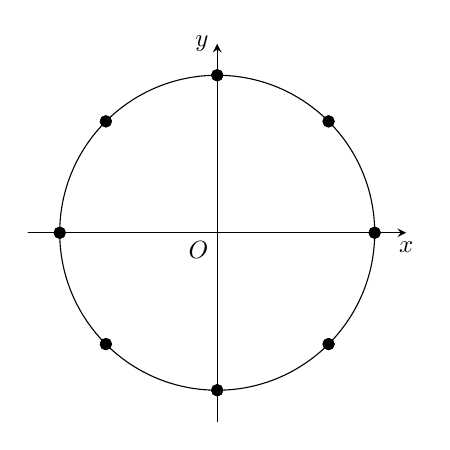
\begin{tikzpicture}[line join=round,line cap=round,>=stealth]
					\tikzset{every node/.style={scale=0.9}} 
					 \draw[->] (-2.4,0)--(2.4,0) node[below] {$x$};
					 \draw[->] (0,-2.4)--(0,2.4) node[left] {$y$};
					\draw (0,0) node [below  left] {$O$};
					\draw (0,0) circle (2); 
					\foreach  \i in {0,...,1}
						 {
					\draw  plot[mark=*] coordinates {({0+\i*360/1}:2)};
					} 
					\foreach \i  in {0,...,1}
						{ 
					\draw plot[mark=*] coordinates  {({-45+\i*360/1}:2)};
					 }
					\foreach \i  in {0,...,1}
						 {
					\draw plot[mark=*] coordinates  {({-90+\i*360/1}:2)};
					 }
					\foreach \i in  {0,...,1}
						 {
					\draw plot[mark=*] coordinates  {({45+\i*360/1}:2)};
					 }
					\foreach \i in  {0,...,1}
						{ 
					\draw  plot[mark=*] coordinates {({90+\i*360/1}:2)};
					 }
					 \foreach \i in {0,...,1}
						 {
					\draw plot[mark=*] coordinates {({135+\i*360/1}:2)}; 
					} 
					\foreach \i  in {0,...,1}
						{ 
					\draw plot[mark=*]  coordinates {({180+\i*360/1}:2)};
					 }
					 \foreach \i in {0,...,1}
						{ 
					\draw plot[mark=*] coordinates  {({225+\i*360/1}:2)};
					} 
				\end{tikzpicture}
		\end{center}
	Vậy có $8$ điểm biểu diễn nghiệm của phương trình trên  trên đường tròn lượng giác.}
\end{ex}

% nguồn: Ok_Toan11_TracNghiem_Lan2
\begin{ex}%[1D1H5-5]%[ma:6f987ff8]
	Số nghiệm của phương trình $3\cot 3x-\sqrt{3}=0$  trên khoảng $\left( -\dfrac{2\pi}{9};\dfrac{\pi}{9} \right)$ là
	\choice 
		{\True $0$} 
		{$1$} 
		 {$2$}
		 {$3$}
	\loigiai{\begin{itemize}
		\item Ta có $\cot  3x=\dfrac{\sqrt{3}}{3}\Leftrightarrow 3x=\dfrac{\pi}{3}+k\pi $, $k\in \mathbb{Z}\Leftrightarrow x=\dfrac{\pi}{9}+\dfrac{k\pi}{3}$, $k\in \mathbb{Z}$.
		\item $x\in \left( -\dfrac{2\pi}{9};\dfrac{\pi}{9} \right)\Leftrightarrow  -\dfrac{2\pi}{9}<\dfrac{\pi}{9}+\dfrac{k\pi}{3}<\dfrac{\pi}{9}\Leftrightarrow -\dfrac{\pi}{3}<\dfrac{k\pi}{3}<0\Leftrightarrow -1<k<0$.
	\end{itemize}
	Vì $k\in \mathbb{Z}$ nên không có giá trị nào của $k$ thỏa  mãn. \\
Vậy  phương trình đã cho không có nghiệm nào trên khoảng $\left( -\dfrac{2\pi}{9};\dfrac{\pi}{9} \right)$.}
\end{ex}

% nguồn: Ok_Toan11_TracNghiem_Lan2
\begin{ex}%[1D1H5-5]%[ma:f48dc985]
	 Tập nghiệm của phương trình $\sin(\pi-x)-\cos\left(\dfrac{\pi}{2}-2x\right)=0$ là
	\choice 
		 {$S=\left\{k2\pi|k\in\mathbb{Z}\right\}$}
		{\True $S=\left\{k2\pi,\dfrac{\pi}{3}+\dfrac{k2\pi}{3}|k\in\mathbb{Z}\right\}$} 
		{$S=\left\{k\pi,\dfrac{\pi}{3}+\dfrac{k2\pi}{3}|k\in\mathbb{Z}\right\}$} 
		 {$S=\left\{\dfrac{\pi}{3}+\dfrac{k2\pi}{3}|k\in\mathbb{Z}\right\}$}
	 \loigiai{
		Ta  có
		\begin{eqnarray*}
			&&\sin(\pi-x)-\cos\left(\dfrac{\pi}{2}-2x\right)=0\Leftrightarrow\sin x-\sin 2x=0\Leftrightarrow\sin 2x=\sin  x\\
			 &\Leftrightarrow&\hoac{&2x=x+k2\pi\\&2x=\pi-x+k2\pi}\Leftrightarrow\hoac{&x=k2\pi\\&x=\dfrac{\pi}{3}+\dfrac{k2\pi}{3}},(k\in\mathbb{Z}).
	\end{eqnarray*}}
\end{ex}

% nguồn: Ok_Toan11_TracNghiem_Lan2
\begin{ex}%[1D1H5-5]%[ma:f5e050e7]
	Các  họ nghiệm của phương trình $\sin 2 x-\sqrt{3}\sin x=0$ là
	 \choice
		{$\hoac{&x=k \pi \\& x= \pm  \dfrac{\pi}{6}+k \pi}$, $k\in\mathbb{Z}$}
		{$x=  \pm \dfrac{\pi}{6}+k \pi$, $k\in\mathbb{Z}$}
		{\True $\hoac{&x=k \pi \\& x= \pm \dfrac{\pi}{6}+k  2 \pi}$, $k\in\mathbb{Z}$}
		{$\hoac{&x=k 2 \pi \\&  x= \pm \dfrac{\pi}{3}+k 2 \pi}$, $k\in\mathbb{Z}$}
	\loigiai{ 
		Ta  có
		\begin{eqnarray*}
			&&\sin 2 x-\sqrt{3}\sin  x=0\\
			&\Leftrightarrow&\sin x(2 \cos x-\sqrt{3})=0\\ 
			&\Leftrightarrow&\hoac{&\sin x=0 \\&  \cos x=\dfrac{\sqrt{3}}{2}}\\
			&\Leftrightarrow&\hoac{&x=k \pi \\& x= \pm \dfrac{\pi}{6}+k 2  \pi.}, k\in\mathbb{Z}
		\end{eqnarray*}
	} 
\end{ex}

% nguồn: Ok_Toan11_TracNghiem_Lan2
\begin{ex}%[1D1H5-5]%[ma:d2e9ea1e]
	Giải  phương trình $\left(2\cos \dfrac{x}{2}-1\right)\left(\sin \dfrac{x}{2}+2\right)=0$
	\choice 
		{$x=\pm \dfrac{2\pi}{3}+k2\pi,  \left(k\in \mathbb{Z}\right)$}
		 {$x=\pm \dfrac{\pi}{3}+k2\pi, \left(k\in \mathbb{Z}\right)$}
		{$x=\pm \dfrac{\pi}{3}+k4\pi,  \left(k\in \mathbb{Z}\right)$}
		{\True $x=\pm  \dfrac{2\pi}{3}+k4\pi, \left(k\in \mathbb{Z}\right)$}
	\loigiai{ 
		Vì  $-1\le \sin \dfrac{x}{2} \le 1, \forall x\in \mathbb{R}\Rightarrow \sin \dfrac{x}{2}+2> 0$.\\
		Vậy phương  trình tương đương
		\begin{eqnarray*}
			& &2\cos  \dfrac{x}{2}-1=0\\
			 &\Leftrightarrow& \cos \dfrac{x}{2}=\dfrac{1}{2}\\
			&\Leftrightarrow&  \dfrac{x}{2}=\pm \dfrac{\pi}{3}+k2\pi\\ &\Leftrightarrow& x=\pm \dfrac{2\pi}{3}+k4\pi,\, \left(k\in \mathbb{Z}\right).
		\end{eqnarray*}
	} 
\end{ex}

% nguồn: Ok_Toan11_TracNghiem_Lan2
\begin{ex}%[1D1H5-5]%[ma:047feab1]
	Nghiệm của phương trình $\sqrt{3}+3  \tan x=0$ là
	\choice 
		{\True $x=-\dfrac{\pi}{6}+k \pi$,  $k \in \mathbb{Z}$}
		{$x=\dfrac{\pi}{2}+k \pi$, $k \in \mathbb{Z}$} 
		{$x=\dfrac{\pi}{3}+k \pi$, $k \in \mathbb{Z}$} 
		{$x=\dfrac{\pi}{2}+k 2 \pi$,  $k \in \mathbb{Z}$}
	\loigiai{Ta có 
		 $$
		\sqrt{3}+3 \tan x=0 \Leftrightarrow \tan x=-\dfrac{\sqrt{3}}{3}\Leftrightarrow  x=-\dfrac{\pi}{6}+k \pi, k \in \mathbb{Z}.
	$$} 
\end{ex}

% nguồn: Ok_Toan11_TracNghiem_Lan2
\begin{ex}%[1D1H5-5]%[ma:d30b244f]
	Giải phương  trình $5 \sin x-\sin 2 x=0$.
	 \choice
		{$x=k 2  \pi$, $(k \in \mathbb{Z})$}
		{$x=\dfrac{\pi}{2}+k \pi $, $(k \in  \mathbb{Z})$}
		 {\True $x=k \pi $, $(k \in \mathbb{Z})$}
		{Phương trình vô nghiệm} 
	 \loigiai{
		 Ta có
		\begin{eqnarray*}
			&&5  \sin x-\sin 2 x=0\\
			&\Leftrightarrow&5  \sin x-2 \sin x \cdot \cos x=0\\
			&\Leftrightarrow&\sin x(5-2  \cos x)=0\\
			&\Leftrightarrow&\hoac{&\sin  x=0 \\& 5-2 \cos x=0.}
		\end{eqnarray*}
		\begin{itemize}
			\item $\sin x=0 \Leftrightarrow x=k \pi$, $(k \in  \mathbb{Z})$.
			\item $5-2 \cos x=0 \Leftrightarrow \cos  x=\dfrac{5}{2}$ (vô nghiệm).
		\end{itemize}
	 }
\end{ex}

% nguồn: Ok_Toan11_TracNghiem_Lan2
\begin{ex}%[1D1H5-5]%[ma:a8329398]
	 Phương trình $\sin x=\cos x$ có số nghiệm thuộc đoạn $\left[-\pi;\pi \right]$ là
	\choice 
		 {$3$}
		{$5$} 
		 {\True $2$}
		 {$4$}
	\loigiai{Ta có $\sin x=\cos x\Leftrightarrow \sqrt{2}\sin \left( x-\dfrac{\pi}{4} \right)=0\Leftrightarrow x-\dfrac{\pi}{4}=k\pi \Leftrightarrow x=\dfrac{\pi}{4}+k\pi,  k\in\mathbb{Z}$.\\
	Trong $\left[-\pi;\pi \right]$ phương  trình có hai nghiệm.}
\end{ex}

% nguồn: Ok_Toan11_TracNghiem_Lan2
\begin{ex}%[1D1H5-5]%[ma:8e821cc8]
	Trên khoảng $\left(\dfrac{\pi}{2}; 2 \pi\right)$, phương trình $\cos \left(\dfrac{\pi}{6}-2 x\right)=\sin x$  có bao nhiêu nghiệm?
	\choice 
		 {$4$}
		{$5$} 
		 {$2$}
		{\True $3$} 
	\loigiai{ 
		 Ta có
		\begin{eqnarray*}
			 &&\cos \left(\dfrac{\pi}{6}-2 x\right)=\sin x\\
			&\Leftrightarrow&\cos \left(\dfrac{\pi}{6}-2 x\right)=\cos \left(\dfrac{\pi}{2}-x\right)\\ 
			&\Leftrightarrow&\hoac{&\dfrac{\pi}{6}-2 x=\dfrac{\pi}{2}-x+k 2 \pi \\& \dfrac{\pi}{6}-2 x=-\dfrac{\pi}{2}+x+k 2 \pi}\\ 
			&\Leftrightarrow&\hoac{&x=-\dfrac{\pi}{3}-k 2 \pi \\& x=\dfrac{2 \pi}{9}-\dfrac{k 2 \pi}{3}}, k \in \mathbb{Z}. 
		\end{eqnarray*}
		Vì $x \in\left(\dfrac{\pi}{2}; 2 \pi\right) \Rightarrow x \in\left\{\dfrac{5 \pi}{3}; \dfrac{8  \pi}{9}; \dfrac{14 \pi}{9}\right\}$.\\
	Vậy phương trình đã  cho có $3$ nghiệm trên khoảng $\left(\dfrac{\pi}{2}; 2 \pi\right)$.}
\end{ex}

% nguồn: Ok_Toan11_TracNghiem_Lan2
\begin{ex}%[1D1H5-5]%[ma:5c97b3a6]
	 Họ nghiệm của phương trình $\tan \left(x-\dfrac{\pi}{4}\right)-1=0$ là
	\choice 
		{\True $x=\dfrac{\pi}{2}+k \pi$, $ k \in  \mathbb{Z}$}
		 {$x=k \pi$, $ k \in \mathbb{Z}$}
		{$x=\dfrac{\pi}{2}+k 2 \pi$,  $ k \in \mathbb{Z}$}
		{$x=\dfrac{\pi}{4}+k \pi$, $  k \in \mathbb{Z}$}
	 \loigiai{
		Ta có $\tan \left(x-\dfrac{\pi}{4}\right)-1=0 \Leftrightarrow \tan \left(x-\dfrac{\pi}{4}\right)=1 \Leftrightarrow  x-\dfrac{\pi}{4}=\dfrac{\pi}{4}+k \pi \Leftrightarrow x=\dfrac{\pi}{2}+k \pi$.\\
	Vậy  nghiệm của phương trình là $x=\dfrac{\pi}{2}+k \pi$, $ k \in \mathbb{Z}$.}
\end{ex}

% nguồn: Ok_Toan11_TracNghiem_Lan2
\begin{ex}%[1D1H5-5]%[ma:b1604384]
	Số vị trí biểu diễn các nghiệm của phương trình $\tan 3x+\cot\left(x-\dfrac{\pi}{2}\right)=0$ trên đường tròn lượng giác  là
	\choice 
		{$4$} 
		 {\True $2$}
		 {$0$}
		 {$1$}
	\loigiai{ 
		Điều kiện $\heva{&\cos  3x\neq 0\\&\sin \left(x-\frac{\pi}{2}\right)\neq 0}\Leftrightarrow\heva{&x\neq\frac{\pi}{6}+\frac{k\pi}{3}\\&x\neq\frac{\pi}{2}+k\pi.} \quad (*)$\\
		 Ta có
		\begin{eqnarray*}
			&&\tan  3x=-\cot\left(x-\dfrac{\pi}{2}\right)\\
			&\Leftrightarrow& \tan  3x=-\tan (-x) \\
			&\Leftrightarrow& \tan  3x=\tan x\\ &\Leftrightarrow& 3x=x+k\pi\\
			&\Leftrightarrow&  x=\dfrac{k\pi}{2}, k\in\mathbb{Z}.
		\end{eqnarray*}
	Kết hợp điều kiện $(*)$ suy ra $x=k\pi, k\in\mathbb{Z}$ nghĩa là có $2$ điểm biểu diễn trên đường tròn lượng giác.} 
\end{ex}

% nguồn: Ok_Toan11_TracNghiem_Lan2
\begin{ex}%[1D1H5-5]%[ma:7d122421]
	Phương trình $\tan \left(3 x-15^{\circ}\right)=\sqrt{3}$ có các nghiệm  là
	\choice 
		{$x=60^{\circ}+k 180^{\circ}$, $k  \in \mathbb{Z}$}
		{$x=75^{\circ}+k 180^{\circ}$,  $k \in \mathbb{Z}$}
		{$x=75^{\circ}+k  60^{\circ}$, $k \in \mathbb{Z}$}
		{\True $x=25^{\circ}+k 60^{\circ}$,  $k \in \mathbb{Z}$}
	 \loigiai{
		 Ta có
		\begin{eqnarray*}
			&&\tan  \left(3 x-15^{\circ}\right)=\sqrt{3}\\
			&\Leftrightarrow&\tan \left(3 x-15^{\circ}\right)=\tan 60^{\circ}\\ 
			 &\Leftrightarrow&3 x-15^{\circ}=60^{\circ}+k 180^{\circ}\\
			&\Leftrightarrow&x=25^{\circ}+k 60^{\circ}, k \in \mathbb{Z}. 
		\end{eqnarray*}
	 }
\end{ex}

% nguồn: Ok_Toan11_TracNghiem_Lan2
\begin{ex}%[1D1H5-5]%[ma:fdfcec2c]
	Giải phương trình $\sin x\sin 7x=\sin 3x\sin  5x$.
	 \choice
		{$x=k\pi, k\in\mathbb{Z}$} 
		 {$x=\dfrac{k\pi}{6}, k\in\mathbb{Z}$}
		{\True $x=\dfrac{k\pi}{4}, k\in\mathbb{Z}$} 
		{$x=\dfrac{k\pi}{2},  k\in\mathbb{Z}$}
	\loigiai{ 
		Ta có 
		\begin{eqnarray*}
			&&\sin  x\sin 7x=\sin 3x\sin 5x\\
			&\Leftrightarrow& \cos  6x-\cos 8x=\cos 2x-\cos 8x\\
			&\Leftrightarrow&  \cos 6x=\cos 2x\\
			&\Leftrightarrow& \hoac{&6x=2x+k2\pi\\&6x=-2x+k2\pi}\\ &\Leftrightarrow& \hoac{&x=\frac{k\pi}{2}\\&x=\frac{k\pi}{4}}\\ &\Leftrightarrow&  x=\dfrac{k\pi}{4}, k\in\mathbb{Z}.
		\end{eqnarray*}
	} 
\end{ex}

% nguồn: Ok_Toan11_TracNghiem_Lan2
\begin{ex}%[1D1H5-5]%[ma:614ba23b]
	Các họ nghiệm của phương trình $\sin 2 x-\sqrt{3}  \sin x=0$ là
	 \def\dotEX{}
	 \choice
		{\True $\hoac{&x=k \pi  \\ &x= \pm \dfrac{\pi}{6}+k \pi.}$}
		{$x= \pm \dfrac{\pi}{6}+k \pi.$} 
		{$\hoac{&x=k \pi \\ &x= \pm  \dfrac{\pi}{6}+k 2 \pi.}$}
		{$\hoac{&x=k 2 \pi \\ &x= \pm \dfrac{\pi}{3}+k  2 \pi.}$}
	 \loigiai{
		\begin{eqnarray*}
			 & &\sin 2 x-\sqrt{3} \sin x=0\\
			&\Leftrightarrow&  \sin x(2 \cos x-\sqrt{3})=0\\
			&\Leftrightarrow& \hoac{&\sin x=0  \\
			&\cos  x=\dfrac{\sqrt{3}}{2}}\\
			&\Leftrightarrow& \hoac{&x=k  \pi \\
			& x= \pm \dfrac{\pi}{6}+k 2 \pi},\,(k\in \mathbb{Z}). 
		\end{eqnarray*}
	} 
\end{ex}

% nguồn: Ok_TracNghiemLop11_Lan1
\begin{ex}%[1D1H5-5]%[ma:23176f5d]
	Nghiệm của phương  trình $\cos \left(\dfrac{x}{2}\right)= -\dfrac{1}{2}$ là
	\choice 
		{\True $x=\dfrac{4\pi}{3}+k2\pi$ hoặc $x=-\dfrac{4\pi}{3} +  k2\pi, \ k\in \mathbb{Z}$}
		{$x=\dfrac{2\pi}{3}  + k2\pi$ hoặc $x=-\dfrac{2\pi}{3} + k2\pi, \ k\in \mathbb{Z}$}
		{$x=\dfrac{4\pi}{3} + k\pi$ hoặc $x=-\dfrac{4\pi}{3} + k\pi, \ k\in \mathbb{Z}$} 
		{$x=\dfrac{2\pi}{6} + k\pi$ hoặc $x=-\dfrac{2\pi}{6} + k\pi, \ k\in  \mathbb{Z}$}
	 \loigiai{
		 Ta có
		$-\dfrac{1}{2} = -\cos \left(\dfrac{\pi}{3}\right) = \cos \left(\pi -  \dfrac{\pi}{3}\right) = \cos \left(\dfrac{2\pi}{3}\right)$.\\
		 Khi đó \\
		\begin{align*}
			&\cos \left(\dfrac{x}{2}\right) = -  \dfrac{1}{2}.\\
			\Leftrightarrow &\cos \left(\dfrac{x}{2}\right) = \cos  \left(\dfrac{2\pi}{3}\right).\\
			\Leftrightarrow&\hoac{&\dfrac{x}{2} = \dfrac{2\pi}{3} + k2\pi\\&\dfrac{x}{2}=-\dfrac{2\pi}{3} +  k2\pi} \\
			\Leftrightarrow &\hoac{&x = \dfrac{4\pi}{3} + k2\pi\\&x=-\dfrac{4\pi}{3} +  k2\pi} \quad k\in \mathbb{Z}.
		\end{align*}
	 }
\end{ex}

% nguồn: Ok_TracNghiemLop11_Lan1
\begin{ex}%[1D1H5-5]%[ma:f6028080]
	Nghiệm của phương trình $\sin 3x = \cos  x$ là
	 \choice
		{$x=k\pi$, $x=\dfrac{\pi}{4}+k\pi$  ($k\in\mathbb{Z}$)}
		{\True $x=\dfrac{\pi}{8}+k\dfrac{\pi}{2}$, $x=\dfrac{\pi}{4}+k\pi$  $(k\in\mathbb{Z})$}
		{$x=k2\pi$, $x=\dfrac{\pi}{2}+k2\pi$ ($k\in\mathbb{Z}$)} 
		{$x=k\pi$, $x=k\dfrac{\pi}{2}$  ($k\in\mathbb{Z}$)}
	 \loigiai{
		Ta  có
		 \allowdisplaybreaks
		\begin{eqnarray*}
			\sin 3x = \cos x 
			&\Leftrightarrow& \sin 3x = \sin \left(\dfrac{\pi}{2}  -x\right) \\
			&\Leftrightarrow& \hoac{&3x =\dfrac{\pi}{2}-x + k2\pi\\&3x =  \dfrac{\pi}{2} + x +k2\pi}\\
			&\Leftrightarrow& \hoac{&x = \dfrac{\pi}{8} + k\dfrac{\pi}{2}\\&x = \dfrac{\pi}{4} + k\pi} \quad (k\in \mathbb{Z}). 
		\end{eqnarray*}
	 }
\end{ex}

% nguồn: Ok_TracNghiemLop11_Lan1
\begin{ex}%[1D1H5-5]%[ma:dbcd18d7]
	Tất cả các nghiệm của  phương trình $\sin 2x-\cos x=0$ là
	 \choice
		 {\True $x=\dfrac{\pi}{2}+k\pi;x=\dfrac{\pi}{6}+k2\pi;x=\dfrac{5\pi}{6}+k2\pi;k\in \mathbb{Z}$}
		{$x=\dfrac{-\pi}{6}+k\dfrac{2\pi}{3};\dfrac{\pi}{2}+k2\pi;x=\dfrac{5\pi}{6}+k2\pi;k\in \mathbb{Z}$} 
		{$x=\dfrac{\pi}{6}+k\dfrac{2\pi}{3};\dfrac{-\pi}{2}+k2\pi;x=\dfrac{5\pi}{6}+k2\pi;k\in \mathbb{Z}$} 
		{$x=\dfrac{-\pi}{6}+k\dfrac{2\pi}{3};\dfrac{-\pi}{2}+k2\pi;x=\dfrac{5\pi}{6}+k2\pi;k\in  \mathbb{Z}$}
	 \loigiai{
		Ta  có
		\allowdisplaybreaks 
		\begin{eqnarray*}
			 &&\sin 2x-\cos x=0\\
			&\Leftrightarrow&\sin  2x=\cos x\\
			 &\Leftrightarrow&\sin 2x=\sin\left(\dfrac{\pi}{2}-x\right)\\
			&\Leftrightarrow&\hoac{&2x=\dfrac{\pi}{2}-x+k2\pi\\&2x=\pi  -\dfrac{\pi}{2}+x+k2\pi}\\
			&\Leftrightarrow&\hoac{&x=\dfrac{\pi}{6}+k\dfrac{2\pi}{3}\\&x=\dfrac{\pi}{2}+k2\pi}\\ 
			&\Leftrightarrow&\hoac{&x=\dfrac{\pi}{2}+k\pi\\&x=\dfrac{\pi}{6}+k2\pi\\&x=\dfrac{5\pi}{6}+k2\pi},k\in \mathbb{Z}. 
		\end{eqnarray*}
	} 
\end{ex}

% nguồn: Ok_TracNghiemLop11_Lan1
\begin{ex}%[1D1H5-5]%[ma:74dda1ec]
	Phương trình $2\sin x -1=0$  có tập nghiệm là
	\choice 
		{$\left\{\dfrac{\pi}3+k 2\pi,-\dfrac{2\pi}3+k 2\pi\text{ với  } k\in\mathbb{Z}\right\}$}
		{\True $\left\{\dfrac{\pi}6+k 2\pi;\dfrac{5\pi}6+k 2\pi  \text{ với } k\in\mathbb{Z}\right\}$}
		{$\left\{\dfrac{\pi}6+k 2\pi;-\dfrac{\pi}6+k 2\pi\text{ với  } k\in\mathbb{Z}\right\}$}
		{$\left\{\dfrac{\pi}2+k 2\pi\text{ với  } k\in\mathbb{Z}\right\}$}
	\loigiai{ 
	$$ 2\sin x -1=0 \Leftrightarrow \sin x=\dfrac{1}{2} \Leftrightarrow \sin x= \sin \dfrac{\pi}{6} \Leftrightarrow \hoac{& x=\dfrac{\pi}{6} +k2\pi, k\in \mathbb{Z} \\ & x=\pi - \dfrac{\pi}{6} +k2\pi , k\in\mathbb{Z}} \Leftrightarrow \hoac{& x=\dfrac{\pi}{6} +k2\pi, k\in \mathbb{Z}  \\ & x=\dfrac{5\pi}{6} +k2\pi , k\in\mathbb{Z}.}$$
	} 
\end{ex}

% nguồn: Ok_TracNghiemLop11_Lan1
\begin{ex}%[1D1H5-5]%[ma:71aa2022]
	Nghiệm của phương trình $2\cos2x  +\sqrt{3}=0$ là
	 \choice
		{ \True  $x=\dfrac{5}{12}\pi + k\pi$, $x=- \dfrac{5}{12}\pi + k\pi(k \in \mathbb{Z})$}
		{ $x=- \dfrac{1}{6}\pi + k\pi$, $x=\dfrac{1}{6}\pi + k\pi(k \in \mathbb{Z})$} 
		{ $x=\dfrac{5}{12}\pi  + k\pi$, $x=- \dfrac{1}{6}\pi + k\pi(k \in \mathbb{Z})$}
		{ $x=\dfrac{5}{6}\pi + k\pi$, $x=- \dfrac{5}{6}\pi + k\pi(k \in  \mathbb{Z})$}
	\loigiai{ 
		$2\cos2x +\sqrt{3}=0\Leftrightarrow \cos  2x=-\dfrac{\sqrt{3}}{2}\Leftrightarrow \hoac{&2x=\dfrac{5\pi}{6}+k2\pi\\&2x=-\dfrac{5\pi}{6}+k2\pi}\Leftrightarrow\hoac{&x=\dfrac{5\pi}{12}+k\pi\\&x=-\dfrac{5\pi}{12}+k\pi}(k\in\mathbb{Z}).$
	} 
\end{ex}

% nguồn: Ok_Toan11_TracNghiem_Lan2
\begin{ex}%[1D1V5-5]%[ma:0f0bd0f4]
	Số điểm phân biệt biểu diễn các nghiệm phương trình $\sin 2x-\sin x=0$ trên đường tròn lượng giác là 
	\choice 
		 {\True $4$}
		 {$1$}
		{$2$} 
		{$3$} 
	 \loigiai{
	 \immini{
		Ta có 
		\begin{eqnarray*}
			& & \sin 2x-\sin x=0\\ 
			&\Leftrightarrow & 2\sin x\cos x-\sin x=0\\ 
			&\Leftrightarrow &  \sin x(2\cos x-1)=0\\
			 &\Leftrightarrow & \hoac{&{\sin x=0} \\
			&{\cos  x=\dfrac{1}{2}.}}
		\end{eqnarray*}
		Các điểm biểu diễn tập nghiệm trên đường tròn lượng  giác như sau
		\begin{itemize}
			\item Các điểm $A,B$ biểu diễn cho nghiệm của phương trình  $\sin x=0$.
			\item Các điểm $C,D$ biểu diễn cho nghiệm  của phương trình $\cos x=\dfrac{1}{2}$.
		\end{itemize}
		Vậy có tất cả $4$ điểm biểu diễn nghiệm của phương trình.} 
		{ 
		\begin{tikzpicture}[line join=round,line cap=round,scale= 0.9]
				\def\r{2} 
				\path 
					 (0,0) coordinate (O)
					(-2,0) coordinate  (B)
					 (2,0) coordinate (A)
					(-2,0)  coordinate (B)
					(60:\r)  coordinate (D)
					 (-60:\r) coordinate (C);
				\draw[->] (-2.5,0)--(2.5,0)  node[below]{$x$};
				\draw[->] (0,-2.5)--(0,2.5)  node[right]{$y$};
				\draw (O) circle (\r); 
				\draw (O)--(D) 
					(O)--(C); 
				\draw[dashed]  (D)--(C);
				 \foreach \x/\g in {O/-135,B/140,A/40,D/45,C/-45}
				 \draw[fill=black](\x) circle (1pt)
					($(\x)+(\g:3mm)$) node{$\x$}; 
			\end{tikzpicture}
		 }
	} 
\end{ex}

% nguồn: Ok_Toan11_TracNghiem_Lan2
\begin{ex}%[1D1V5-5]%[ma:c9e2ed53]
	Số nghiệm phương trình $\dfrac{\sin 3x}{\cos x+1}=0$  thuộc đoạn $\left[2\pi;4\pi \right]$ là
	\choice 
		 {$8$}
		 {$7$}
		{\True $6$} 
		{$5$} 
	\loigiai{ 
		Điều kiện $\cos  x+1\ne 0\Leftrightarrow x\ne \pi+k2\pi$.\\
		Ta  có $\dfrac{\sin 3x}{\cos x+1}=0\Rightarrow \sin 3x=0\Leftrightarrow x=\dfrac{k\pi}{3}, (k\in \mathbb{Z})$.\\
		So với điều kiện nghiệm của phương trình là  $x=\dfrac{k\pi}{3}$ với $k\in \mathbb{Z}$, $k\ne 3(2l+1)$.\\
		 Vì $2\pi \le x\le 4\pi \Leftrightarrow 2\pi \le \dfrac{k\pi}{3} \le 4\pi \Leftrightarrow 6\le k\le 12$ nên ta chọn $k\in \left\{6,7,8,10,11,12\right\}$.\\
	Vậy  có $6$ nghiệm thuộc đoạn $\left[2\pi;4\pi \right]$.}
\end{ex}

% nguồn: Ok_Toan11_TracNghiem_Lan2
\begin{ex}%[1D1V5-5]%[ma:2883ac09]
	Phương trình $\sin x=\cos x$ có bao nhiêu nghiệm $x\in \left(0;5\pi  \right)$?
	\choice 
		{$3$} 
		 {$4$}
		 {\True $5$}
		 {$6$}
	\loigiai{ 
		Ta  có
		\begin{eqnarray*}
			&&\sin x=\cos x\\ 
			&\Leftrightarrow& \tan  x=1\\
			&\Leftrightarrow& x=\dfrac{\pi}{4}+k\pi,\,  k\in {\bf \mathbb{Z}}.
		\end{eqnarray*}
		 Vì $x\in \left(0;5\pi \right)$ nên ta có
		\begin{eqnarray*}
			 &&0< \dfrac{\pi}{4}+k\pi < 5\pi, k\in {\bf \mathbb{Z}}\\
			&\Leftrightarrow&-\dfrac{1}{4} < k  < \dfrac{19}{4}, k\in {\bf \mathbb{Z}}.
		\end{eqnarray*}
		Do đó,  $k\in \left\{0,1, 2,3, 4\right\}$.\\
		Suy ra phương trình  có $5$ nghiệm thuộc $\left(0;5\pi \right)$ là $\dfrac{\pi}{4}$, $\dfrac{5\pi}{4}$, $\dfrac{9\pi}{4}$, $\dfrac{13\pi}{4}$, $\dfrac{17\pi}{4}$.
	 }
\end{ex}

% nguồn: Ok_Toan11_TracNghiem_Lan2
\begin{ex}%[1D1V5-5]%[ma:ebae772e]
	Tập nghiệm của phương trình $\sin\left(\pi x\right)=\cos\left(\dfrac{\pi}{3}+\pi x\right)$  là
	\choice 
		 {$\left\{\dfrac{\pi}{12}+k\pi ,k\in\mathbb{Z}\right\}$}
		 {\True $\left\{\dfrac{1}{12}+k,k\in\mathbb{Z}\right\}$}
		{$\left\{\dfrac{\pi}{2}+k\pi ,k\in\mathbb{Z}\right\}$} 
		 {$\left\{\dfrac{1}{2}+k\pi ,k\in\mathbb{Z}\right\}$}
	 \loigiai{
		 Ta có
		\begin{eqnarray*}
			 \sin\left(\pi x\right)=\cos\left(\dfrac{\pi}{3}+\pi x\right)&\Leftrightarrow&\sin\left(\pi x\right)=\sin\left(\dfrac{\pi}{2}-\dfrac{\pi}{3}-\pi x\right)\Leftrightarrow\sin\left(\pi x\right)=\sin\left(\dfrac{\pi}{6}-\pi x\right)\\
			&\Leftrightarrow&\hoac{&\pi x=\dfrac{\pi}{6}-\pi x+k2\pi\\&\pi x=\pi-\dfrac{\pi}{6}+\pi  x+k2\pi}\Leftrightarrow x=\dfrac{1}{12}+k\,(k\in\mathbb{Z}).
		\end{eqnarray*}
		Vậy tập nghiệm của  phương trình đã cho là $\left\lbrace \dfrac{1}{12}+k,k\in\mathbb{Z}\right\rbrace$.
	} 
\end{ex}

% nguồn: Ok_Toan11_TracNghiem_Lan2
\begin{ex}%[1D1V5-5]%[ma:1be8047b]
	Tập nghiệm của phương trình  $\sin x=2\cos x$ là
	 \choice
		{\True $S=\left\lbrace\arctan 2+k\pi\mid  k\in\mathbb{Z}\right\rbrace$}
		 {$S=\varnothing$}
		{$S=\left\lbrace k\pi\mid k\in\mathbb{Z}\right\rbrace$} 
		{$S=\left\lbrace  \tan 2+k\pi\mid k\in\mathbb{Z}\right\rbrace$}
	\loigiai{ 
		Ta có $\sin  x=2\cos x$.\\
		Với $\cos x=0$ thay vào phương trình, ta thấy vô nghiệm.\\ 
		 Với $\cos x\neq 0\Leftrightarrow x\neq\dfrac{\pi}{2}+k\pi, k\in\mathbb{Z}$ thì ta có $\tan x=2\Leftrightarrow x=\arctan2+k\pi,k\in\mathbb{Z}$.\\
		So  với điều kiện ta có tập nghiệm của phương trình là $S=\left\lbrace \arctan 2+k\pi\mid k\in\mathbb{Z}\right\rbrace$.
	} 
\end{ex}

% nguồn: Ok_Toan11_TracNghiem_Lan2
\begin{ex}%[1D1V5-5]%[ma:713467a2]
	Cho phương trình $\sqrt{3}\tan  2x=3$ có nghiệm $x_0$. Khi đó $\cos x_0$ nhận giá trị là
	 \choice
		 {$\dfrac{-\sqrt{3}}{2}$}
		{\True $\pm\dfrac{\sqrt{3}}{2}$;  $\pm\dfrac{1}{2}$}
		 {$\pm\dfrac{\sqrt{3}}{2}$}
		 {$\pm\dfrac{1}{2}$}
	\loigiai{ 
		Ta có $\sqrt{3}\tan 2x=3\Leftrightarrow\tan 2x=\dfrac{3}{\sqrt{3}}\Leftrightarrow 2x=\dfrac{\pi}{3}+k\pi\Leftrightarrow x=\dfrac{\pi}{6}+\dfrac{k\pi}{2}, k\in\mathbb{Z}$.\\ 
		Suy  ra $x_0\in\left\lbrace\dfrac{\pi}{6}+k2\pi;\dfrac{2\pi}{3}+k2\pi;\dfrac{7\pi}{6}+k2\pi;\dfrac{5\pi}{3}+k2\pi\mid k\in\mathbb{Z}\right\rbrace$.\\ Vậy $\cos x_0\in\left\lbrace\pm\dfrac{\sqrt{3}}{2};\pm\dfrac{1}{2}\right\rbrace$.
	 }
\end{ex}

% nguồn: Ok_Toan11_TracNghiem_Lan2
\begin{ex}%[1D1V5-5]%[ma:ef7f9716]
	Phương trình $\sin 5x-\sin x=0$ có bao nhiêu nghiệm thuộc đoạn $[-2018\pi;2018\pi]$? 
	\choice 
		{$20179$} 
		 {$20181$}
		{$16144$} 
		 {\True $16145$}
	 \loigiai{
		 Ta có
		\begin{eqnarray*}
			\sin 5 x-\sin x=0  &\Leftrightarrow& \sin 5x=\sin x \\ &\Leftrightarrow&\hoac{
			5x &= x  + k2\pi \\
			5x &= \pi  - x + k2\pi }\\
			&\Leftrightarrow&  \hoac{
			& x=k\dfrac{\pi}{2} \\ 
			& x=\dfrac{\pi}{6}+k \dfrac{\pi}{3}}\\ 
			&\Leftrightarrow&  \hoac{
			& x=k\dfrac{\pi}{2} \, (k \in \mathbb{Z})  \\
			& x=\dfrac{5 \pi}{6}+m  \pi \, (m \in \mathbb{Z}) \\
			& x=\dfrac{\pi}{6}+n  \pi \, (n \in \mathbb{Z}).
			} 
		\end{eqnarray*}
		Vì $x \in[-2018\pi;2018\pi]$  nên $\hoac{
		&-2018 \pi \leq k \dfrac{\pi}{2} \leq 2018\pi  \\
		&-2018 \pi \leq \dfrac{5 \pi}{6}+m \pi \leq 2018\pi  \\
		&-2018 \pi \leq \dfrac{\pi}{6}+n  \pi \leq 2018\pi}
		\Leftrightarrow  \hoac{
		&-4036 \leq  k \leq 4036 \\
		&-\dfrac{12113}{6} \leq m \leq  \dfrac{12103}{6} \\
		&-\dfrac{12109}{6} \leq n \leq \dfrac{12107}{6}.}$\\ 
		Do đó  có $8073$ giá trị $k$, $4036$ giá trị $m$, $4036$ giá trị $n$, suy ra số nghiệm cần tìm là $16145$ nghiệm.
	} 
\end{ex}

% nguồn: Ok_Toan11_TracNghiem_Lan2
\begin{ex}%[1D1V5-5]%[ma:ca1e96bc]
	Nghiệm của phương trình $\sin 3x=\cos  x$ là
	 \choice
		{$x=k\pi$; $x=k\dfrac{\pi}{2}$} 
		{\True $x=\dfrac{\pi}{8}+k\dfrac{\pi}{2}$;  $x=\dfrac{\pi}{4}+k\pi$}
		 {$x=k2\pi$; $x=\dfrac{\pi}{2}+k2\pi$}
		{$x=k\pi$; $x=\dfrac{\pi}{4}+k\pi$} 
	\loigiai{ 
		Ta  có
		\begin{eqnarray*}
			 &&\sin 3x=\cos x\\
			&\Leftrightarrow& \sin  3x=\sin \left(\dfrac{\pi}{2}-x\right)\\
			&\Leftrightarrow& \hoac{&{3x=\dfrac{\pi}{2}-x+k2\pi} \\ 
			 &{3x=\pi-\dfrac{\pi}{2}+x+k2\pi}}\\
			 &\Leftrightarrow& \hoac{&{x=\dfrac{\pi}{8}+k\dfrac{\pi}{2}} \\
			&{x=\dfrac{\pi}{4}+k\pi}},\,(k\in  \mathbb{Z}).
		\end{eqnarray*}
	} 
\end{ex}

% nguồn: Ok_Toan11_TracNghiem_Lan2
\begin{ex}%[1D1V5-5]%[ma:b709ce24]
	Hỏi trên $\left[0;\dfrac{\pi}{2}\right]$, phương trình $\sin x=\dfrac{1}{2}$  có bao nhiêu nghiệm?
	\choice 
		{\True  $1$}
		 {$2$}
		{$3$} 
		 {$4$}
	 \loigiai{
		 Ta có $\sin x=\dfrac{1}{2}
		 \Leftrightarrow
		\hoac{&x=\dfrac{\pi}{6}+k2\pi\\ 
		&x=\dfrac{5\pi}{6}+k2\pi}\left(k\in\mathbb{Z}\right)$.\\ 
		Trên đoạn $\left[0;\dfrac{\pi}{2}\right]$ chỉ có một  nghiệm $x=\dfrac{\pi}{6}$ thoả mãn.
	} 
\end{ex}

% nguồn: Ok_Toan11_TracNghiem_Lan2
\begin{ex}%[1D1V5-5]%[ma:6962d257]
	Phương trình $\sin 2x+\cos x=0$ có tổng các nghiệm trong khoảng $\left(0;  2\pi \right)$ bằng
	\choice 
		{$2\pi$} 
		 {$3\pi$}
		{\True  $5\pi$}
		{$6\pi$} 
	 \loigiai{
		 Ta có
		\begin{eqnarray*}
			&&\sin 2x+\cos  x=0\\
			&\Leftrightarrow&  2\sin x\cos x+\cos x=0\\
			&\Leftrightarrow&  \hoac{&{\cos x=0} \\
			&{2\sin  x+1=0}}\\
			 &\Leftrightarrow& \hoac{&{x=\dfrac{\pi}{2}+k\pi} \\
			 &{x=-\dfrac{\pi}{6}+k2\pi} \\
			 &{x=\dfrac{7\pi}{6}+k2\pi}
			}, \left(k\in \mathbb{Z}\right) 
		\end{eqnarray*}
		Vì $x\in \left(0; 2\pi \right)\Rightarrow x=\left\{\dfrac{\pi}{2}; \dfrac{3\pi}{2}; \dfrac{11\pi}{6}; \dfrac{7\pi}{6} \right\}\Rightarrow S=5\pi.$ 
	} 
\end{ex}

% nguồn: Ok_TracNghiemLop11_Lan1
\begin{ex}%[1D1V5-5]%[ma:8b3f84e3]
	Số nghiệm  của phương trình $\sin2x+\cos x=0$ trên $\left[0;2\pi\right]$ là
	\choice 
		{$3$} 
		 {$1$}
		{$2$} 
		{\True $4$} 
	 \loigiai{
		\begin{eqnarray*}
			\sin 2x+\cos x=0 &\Leftrightarrow & 2\sin x\cdot \cos x+\cos  x=0\\
			 &\Leftrightarrow& \cos x(2\sin x+1)=0\\
			 &\Leftrightarrow& \hoac{& \sin x=-\dfrac{1}{2}\\& \cos x=0} \Leftrightarrow \hoac{& x=-\dfrac{\pi}{6}+k2\pi\\& x=\dfrac{7\pi}{6}+k2\pi \\& x=\dfrac{\pi}{2}+k\pi},\,\,(k\in \mathbb{Z}).
		\end{eqnarray*}
		\begin{itemize}
			\item  TH1: $x=-\dfrac{\pi}{6}+k2\pi,k\in \mathbb{Z}$.\\
			Do $x\in  \left[0;2\pi\right]$ nên $\heva{&0\le -\dfrac{\pi}{6}+k2\pi \le 2\pi\\&k\in \mathbb{Z}}\Leftrightarrow \heva{&\dfrac{1}{12}\le k\le \dfrac{13}{12}\\&k\in \mathbb{Z}}\Leftrightarrow k=1$. \\
			Nghiệm của phương trình trong trường hợp  này là $x=\dfrac{11\pi}{6}$.
			\item TH2: $x=\dfrac{7\pi}{6}+k2\pi,k\in  \mathbb{Z}$.\\
			 Do $x\in \left[0;2\pi\right]$ nên $\heva{&0\le \dfrac{7\pi}{6}+k2\pi \le 2\pi\\&k\in \mathbb{Z}}\Leftrightarrow \heva{&-\dfrac{7}{12}\le k\le \dfrac{5}{12}\\&k\in \mathbb{Z}}\Leftrightarrow k=0$. \\
			 Nghiệm của phương trình trong trường hợp này là $x=\dfrac{7\pi}{6}$.\\
			\item TH3: $x=\dfrac{\pi}{2}+k\pi,k\in \mathbb{Z}$.\\ 
			Do $x\in \left[0;2\pi\right]$ nên  $\heva{&0\le \dfrac{\pi}{2}+k\pi \le 2\pi\\&k\in \mathbb{Z}}\Leftrightarrow \heva{&-\dfrac{1}{2}\le k\le \dfrac{3}{2}\\&k\in \mathbb{Z}}\Leftrightarrow k\in \left\{0;1\right\}$. \\
			Nghiệm của phương trình trong  trường hợp này là $x=\dfrac{\pi}{2},x=\dfrac{3\pi}{2}$.
		\end{itemize}
	Vậy các nghiệm thỏa mãn yêu cầu bài toán là $\dfrac{\pi}{2}$; $\dfrac{3\pi}{2}$;  $\dfrac{7\pi}{6}$; $\dfrac{11\pi}{6}$.}
\end{ex}


%%%%%%%%%%%%%%%% ĐÚNG/SAI %%%%%%%%%%%%%%%%

% nguồn: Ok_dungsai_lop11_Lan1
\begin{ex}%[1D1N5-5]%[ma:dec3ab06]
 Cho hàm số $y = \sin x$.  Khi đó
  \choiceTF
  {\True $\sin  x < 0 $ khi $ -\dfrac{\pi}{2} < x < 0$}
  {\True Hàm số $y = \sin x$ là hàm số lẻ với mọi $x  \in \mathbb{R}$}
  {Phương trình $\sin x  = 1$ có nghiệm $x=\dfrac{\pi}{2} + k\pi,\ k\in \mathbb{Z}$}
  {Hàm số $y=\sin x$ có  chặn dưới là $0$}
 \loigiai{ 
  \begin{itemchoice}
   \itemch Đúng. Vì $x$ thuộc gốc  phần tư thứ tư nên $\sin x < 0 $.
   \itemch Đúng. Vì $f(-x) = \sin\left(x\right) = - \sin x  = -f(x)$.
   \itemch Sai.\\ 
   \begin{align*}
    &\sin x =  1\\
    \Leftrightarrow &x = \dfrac{\pi}{2} + k\mathbf{2}\pi\ \forall k \in  \mathbb{Z}.
   \end{align*}
   \itemch Sai. Vì $-1 \le \sin x \le 1$ nên hàm số  có chặn dưới là $-1$.
  \end{itemchoice}
  }
\end{ex}

% nguồn: Ok_dungsai_lop11_Lan1
\begin{ex}%[1D1N5-5]%[ma:fd8e213c]
 \immini{ 
 Điểm nào trong hình bên biểu diễn nghiệm của  phương trình $2\sin x+1=0$?
 \choiceTF 
  {\True  Điểm $E$}
  {Điểm $D$} 
   {Điểm $C$}
   {\True Điểm $F$}
  }{\begin{tikzpicture}[>=stealth,line join=round,line cap=round,font=\footnotesize,scale=1.2]
  \draw[->] (-1.3,0)--(1.3,0) node[right]  {$x$};
   \draw[->] (0,-1.3)--(0,1.3) node[above] {$y$};
  \path 
   (0:0)  coordinate (O)++(0:1) coordinate (A)
   (O)++(30:1) coordinate (C) 
    (O)++(90:1) coordinate (B)
    (O)++(150:1) coordinate (D)
   (O)++(180:1)  coordinate (A')
    (O)++(-150:1) coordinate (E)
   (O)++(-90:1) coordinate  (B')
   (O)++(-30:1) coordinate  (F);
   \draw (C)--(E)
    (D)--(F);
  \draw[dashed]  (C)--(D)
    (E)--(F);
  \draw (O) circle (1); 
  \foreach\p /\r in  {A/45,B/45,C/45,D/135,E/-135,F/-45,A'/135,B'/-45,O/-120}
  \fill (\p)  circle (1.2pt) node[shift={(\r:3mm)}]{$\p$};
   \fill (0,0.5) node[above right]{\footnotesize{$\tfrac{1}{2}$}}circle (1.2pt)
   (0,-0.5)  node[below right]{\footnotesize{$-\tfrac{1}{2}$}}circle (1.2pt);
 \end{tikzpicture}
  } 
 \loigiai{ 
  Các  điểm biểu diễn nghiệm của phương trình $2\sin x+1=0$ là các điểm có tung độ bằng $-\dfrac{1}{2}$ và là các điểm $E$ và $F$.
  }
\end{ex}

% nguồn: Ok_dungsai_lop11_Lan1
\begin{ex}%[1D1H5-5]%[ma:985739d1]
 Cho phương trình lượng giác $2  \cos \left(x+\dfrac{\pi}{3}\right)-m+1=0$, trong đó $m \in \mathbb{R}$ là tham số. Xét tính đúng - sai của các phát biểu sau.
  \choiceTF
  {\True Khi $m=0$ phương trình có tập nghiệm là $\left\{\dfrac{\pi}{3}+k 2 \pi;-\pi+k  2 \pi \bigg| k \in \mathbb{Z}\right\}$}
  { Tập các giá trị  của $m$ để phương trình có nghiệm là $[-1; 1]$}
  {\True  $\dfrac{\pi}{6}$ là nghiệm của phương trình khi và chỉ khi $m=1$}
  {\True Khi  $m=1$ phương trình có $6$ nghiệm trong đoạn $[0; 6 \pi]$}
  \loigiai{
  \begin{itemchoice}
   \itemch Đúng. Với $m=0$ phương  trình trở thành
   \begin{align*}
    2 \cos \left(x+\dfrac{\pi}{3}\right)+1=0 &\Leftrightarrow \cos  \left(x+\dfrac{\pi}{3}\right)=-\dfrac{1}{2}\\
    &\Leftrightarrow \cos \left(x+\dfrac{\pi}{3}\right)=\cos \dfrac{2 \pi}{3}\\ 
     &\Leftrightarrow\hoac{
    &x+\dfrac{\pi}{3}=\dfrac{2 \pi}{3}+k 2 \pi  \\ &x+\dfrac{\pi}{3}=-\dfrac{2 \pi}{3}+k 2 \pi}\\
    &\Leftrightarrow\hoac{&x=\dfrac{\pi}{3}+k 2 \pi  \\ &x=-\pi+k 2 \pi} (k\in\mathbb{Z}).
   \end{align*}
   \itemch $2  \cos \left(x+\dfrac{\pi}{3}\right)-m+1=0 \Leftrightarrow \cos \left(x+\dfrac{\pi}{3}\right)=\dfrac{1-m}{2}$.\\
   Phương trình trên có nghiệm khi và chỉ khi $$-1 \leq \dfrac{1-m}{2} \leq  1 \Leftrightarrow-2 \leq 1-m \leq 2 \Leftrightarrow-1 \leq m \leq 3.$$
   \itemch Đúng. $\dfrac{\pi}{6}$ là nghiệm của phương trình khi và chỉ khi $$2 \cos  \left(\dfrac{\pi}{6}+\dfrac{\pi}{3}\right)-m+1=0 \Leftrightarrow-m+1=0 \Leftrightarrow m=1.$$
   \itemch Với $m=1$ phương trình trở thành 
   $$\cos \left(x+\dfrac{\pi}{3}\right)=0 \Leftrightarrow x+\dfrac{\pi}{3}=\dfrac{\pi}{2}+k \pi \Leftrightarrow  x=\dfrac{\pi}{6}+k \pi,k \in \mathbb{Z}.$$
   Theo bài ra $x \in[0; 6  \pi] \Leftrightarrow 0 \leq \dfrac{\pi}{6}+k \pi \leq 6 \pi \Leftrightarrow-\dfrac{\pi}{6} \leq k \pi \leq \dfrac{35 \pi}{6} \Leftrightarrow-\dfrac{1}{6} \leq k \leq \dfrac{35}{6}$.\\
   Mà $k \in \mathbb{Z}$  nên $k \in\{0; 1; 2; 3; 4; 5\}$.\\
   Suy ra phương trình có $6$ nghiệm trong đoạn $[0; 6  \pi]$
  \end{itemchoice}
  }
\end{ex}

% nguồn: Ok_dungsai_lop11_Lan1
\begin{ex}%[1D1H5-5]%[ma:28b73342]
 Cho hàm số $y=\cos  2x$. Các mệnh đề sau đúng hay sai?
  \choiceTF
  {\True $\cos 2x=2\cos^2x  -1$}
  {Hàm số $g(x)=\cos  2x$ là hàm số lẻ}
   {Phương trình $\cos 2x=0\Leftrightarrow \hoac{&\cos x=1\\&\cos x=-1}$}
  {\True Đồ thị  hàm số $y=\cos 2x$ cắt trục $Ox$ tại $4$ điểm phân biệt trên đoạn $\left[0;2\pi\right]$}
  \loigiai{
  \begin{itemchoice}
    \itemch Áp dụng công thức nhân đôi
   $$\cos  2\alpha=\cos^2\alpha-\sin^2\alpha=2\cos^2\alpha-1=1-2\sin^2\alpha.$$
   \itemch Ta có $\heva{&\forall x\in\mathscr{D}\Rightarrow -x\in \mathscr{D}\\&g(-x)=\cos 2(-x)=2\cos^2(-x)  -1=2\cos^2x -1=g(x)}$.\\
   Vậy hàm  số $g(x)=\cos 2x$ là hàm số chẵn.
   \itemch Ta có $\cos 2x=0\Leftrightarrow 2\cos^2x -1=0\Leftrightarrow \cos^2x =\dfrac{1}{2}\Leftrightarrow\hoac{&\cos  x=\dfrac{1}{\sqrt{2}}\\&\cos x=-\dfrac{1}{\sqrt{2}}.}$
   \itemch  \immini
    {
   Phương trình hoành độ giao điểm  của đồ thị hàm số $y=\cos 2x$ và trục $Ox$ là $$\cos 2x=0\Leftrightarrow\hoac{&\cos x=\dfrac{1}{\sqrt{2}}\ \ \ (1)\\&\cos x=-\dfrac{1}{\sqrt{2}}\ \ \ (2).}$$
   Dựa vào đường tròn lượng giác, mỗi phương trình $(1)$, $(2)$ đều có  $2$ nghiệm phân biệt trên đoạn $\left[0;2\pi\right]$.\\
   Vậy đồ thị  hàm số $y=\cos 2x$ cắt trục $Ox$ tại $4$ điểm phân biệt trên đoạn $\left[0;2\pi\right]$.
   } 
    {
   \begin{tikzpicture}[>=stealth,line join=round,line cap=round,font=\footnotesize,scale=0.7]
     \draw [->] (-3,0)--(3,0); 
      \draw[->] (0,-3)--(0,3);
     \draw (0,0) node[below right]{$O$} coordinate (O) circle  (1pt);
     \draw (3,0) node[below]{$\cos  x$};
     \draw (0,3) node[right]{$\sin x$}; 
     \draw[black]  (0,0) circle (2cm);
     \draw (-0.707,-3)--(-0.707,3); 
     \draw (0.707,-3)--(0.707,3); 
     \draw (0.707,0) node[below right]{$\dfrac{1}{\sqrt{2}}$} coordinate (O) circle  (1pt);
      \draw (-0.707,0) node[below left]{$\dfrac{-1}{\sqrt{2}}$} coordinate (O) circle (1pt);
    \end{tikzpicture}
    }
  \end{itemchoice}
 } 
\end{ex}

% nguồn: Ok_dungsai_lop11_Lan1
\begin{ex}%[1D1H5-5]%[ma:9b40061d]
 Cho phương trình $\sin \left(2 x+\dfrac{\pi}{3}\right)=\dfrac{1}{2}$. Xét tính đúng  sai của các mệnh đề sau.
 \choiceTF 
  {\True Phương trình đã cho có $2$ nghiệm trên khoảng $(0; \pi)$} 
  {\True Số vị trí  biểu diễn các nghiệm của phương trình đã cho trên đường tròn lượng giác là $4$}
  {Tổng tất cả các nghiệm của phương trình  đã cho trên khoảng $(0; \pi)$ bằng $0$}
   {\True Phương trình đã cho có $4$ nghiệm trên khoảng $(0; 2 \pi)$}
 \loigiai{ 
  Ta có $\begin{aligned}
  \sin \left(2 x+\dfrac{\pi}{3}\right)=\dfrac{1}{2} &\Leftrightarrow \sin \left(2  x+\dfrac{\pi}{3}\right)=\sin \dfrac{\pi}{6}\\
  & \Leftrightarrow\hoac{&2  x+\dfrac{\pi}{3}=\dfrac{\pi}{6}+k 2 \pi \\ &2 x+\dfrac{\pi}{3}=\pi-\dfrac{\pi}{6}+k 2 \pi}\\
  &\Leftrightarrow\hoac{&x=-\dfrac{\pi}{12}+k \pi \\ & x=\dfrac{\pi}{4}+k \pi},(k \in \mathbb{Z}). 
 \end{aligned}$\\
 Biểu diễn nghiệm $x=-\dfrac{\pi}{12}+k \pi$ trên đường tròn lượng giác ta được  $2$ vị trí (hình 1).\\
 Biểu diễn nghiệm $x=\dfrac{\pi}{4}+k \pi$  trên đường tròn lượng giác ta được $2$ vị trí (hình 2).
 \begin{center}
  \begin{tikzpicture}[scale=1,font=\footnotesize,line join=round,line cap=round,>=stealth]<DTools>
    \def\xmin{-3.5};  \def\ymin{-3.5}; \def\xmax{3.3}; \def\ymax{3.5};
     \coordinate (O) at (0,0);
    \draw[->] (\xmin,0)--(\xmax,0)  node[below]{$x$};
    \draw[->]  (0,\ymin)--(0,\ymax) node[left]{$y$};
    \fill (O) node[below left]{$O$}  circle (1pt);
    \draw (O) circle  (2.5 cm);
    \coordinate (t) at ($(O) +  (-15:2.5)$);
    \coordinate (t')  at ($(O) + (165:2.5)$);
    \draw[dashed] (t) node [right]{$-\dfrac{\pi}{12}$}--(t')  node [left]{$\dfrac{11\pi}{12}$};
    \draw (0,-4) node {Hình  1};
   \end{tikzpicture}
  \begin{tikzpicture}[scale=1,font=\footnotesize,line join=round,line cap=round,>=stealth]
    \def\xmin{-3.5}; \def\ymin{-3.5}; \def\xmax{3.3}; \def\ymax{3.5}; 
    \coordinate (O) at  (0,0);
    \draw[->] (\xmin,0)--(\xmax,0)  node[below]{$x$};
    \draw[->] (0,\ymin)--(0,\ymax)  node[left]{$y$};
    \fill (O) node[above left]{$O$} circle (1pt); 
    \draw (O)  circle (2.5 cm);
    \coordinate (t)  at ($(O) + (45:2.5)$);
    \coordinate (t') at ($(O)  + (225:2.5)$);
    \draw[dashed]  (t) node [right]{$\dfrac{\pi}{4}$}--(t') node [left]{$\dfrac{5\pi}{4}$};
    \draw  (0,-4) node {Hình 2};
   \end{tikzpicture}
 \end{center}
 \begin{itemchoice}
  \itemch Đúng. Phương trình đã cho có 2 nghiệm trên khoảng  $(0; \pi)$ là $\dfrac{\pi}{4}$, $\dfrac{11 \pi}{12}$.
  \itemch Đúng.  Số vị trí biểu diễn các nghiệm của phương trình $\sin \left(2 x+\dfrac{\pi}{3}\right)=\dfrac{1}{2}$ trên đường tròn lượng giác là $4$.
  \itemch Sai. Tổng tất cả các nghiệm của phương trình đã  cho trên khoảng $(0; \pi)$ bằng $\dfrac{7 \pi}{6}$.
  \itemch Đúng. Phương trình đã cho có $4$ nghiệm trên khoảng  $(0; 2 \pi)$ là $\dfrac{\pi}{4}$, $\dfrac{5 \pi}{4}$, $\dfrac{11 \pi}{12}$, $\dfrac{23 \pi}{12}$.
 \end{itemchoice}
 }
\end{ex}

% nguồn: Ok_dungsai_lop11_Lan1
\begin{ex}%[1D1H5-5]%[ma:bed1fff3]
 Cho phương trình $\sin \left(2 x+\dfrac{\pi}{3}\right)=\dfrac{1}{2}$.  Xét tính đúng sai của các mệnh đề sau.
 \choiceTF 
  {\True Số điểm biểu  diễn các nghiệm của phương trình trên đường tròn lượng giác là $4$}
   {\True Phương trình đã cho có $2$ nghiệm trên khoảng $(0; \pi)$}
  {Tổng  tất cả các nghiệm của phương trình đã cho trên khoảng $(0; \pi)$ bằng $0$}
   {\True Phương trình đã cho có $4$ nghiệm trên khoảng $(0; 2 \pi)$}
  \loigiai{
  Ta có $\begin{aligned}
  \sin \left(2 x+\dfrac{\pi}{3}\right)=\dfrac{1}{2} &\Leftrightarrow  \sin \left(2 x+\dfrac{\pi}{3}\right)=\sin \dfrac{\pi}{6}\\
  & \Leftrightarrow\hoac{&2 x+\dfrac{\pi}{3}=\dfrac{\pi}{6}+k 2 \pi \\ &2 x+\dfrac{\pi}{3}=\pi-\dfrac{\pi}{6}+k 2 \pi}\\ 
  &\Leftrightarrow\hoac{&x=-\dfrac{\pi}{12}+k \pi \\ & x=\dfrac{\pi}{4}+k  \pi},(k \in \mathbb{Z}).
 \end{aligned}$\\
 Biểu diễn nghiệm $x=-\dfrac{\pi}{12}+k \pi$ trên đường  tròn lượng giác ta được $2$ vị trí (hình 1).\\
 Biểu diễn nghiệm $x=\dfrac{\pi}{4}+k \pi$ trên đường tròn lượng giác ta được  $2$ vị trí (hình 2).
 \begin{center}
  \begin{tikzpicture}[scale=0.8,font=\footnotesize,line join=round,line cap=round,>=stealth]
    \def\xmin{-3.5}; \def\ymin{-3.5}; \def\xmax{3.3}; \def\ymax{3.5}; 
    \coordinate  (O) at (0,0);
    \draw[->] (\xmin,0)--(\xmax,0) node[above]{$x$}; 
     \draw[->] (0,\ymin)--(0,\ymax) node[left]{$y$};
    \fill  (O) node[below left]{$O$} circle (1pt);
    \draw (O) circle (2.5 cm); 
     \coordinate (t) at ($(O) + (-15:2.5)$);
    \coordinate (t') at  ($(O) + (165:2.5)$);
    \draw[dashed] (t)  node [right]{$-\dfrac{\pi}{12}$}--(t') node [left]{$\dfrac{11\pi}{12}$};
     \draw (0,-4) node {Hình 1};
   \end{tikzpicture}
  \begin{tikzpicture}[scale=0.8,font=\footnotesize,line join=round,line cap=round,>=stealth]
    \def\xmin{-3.5}; \def\ymin{-3.5}; \def\xmax{3.3}; \def\ymax{3.5}; 
    \coordinate  (O) at (0,0);
     \draw[->] (\xmin,0)--(\xmax,0) node[below]{$x$};
    \draw[->] (0,\ymin)--(0,\ymax) node[left]{$y$}; 
     \fill (O) node[above left]{$O$} circle (1pt);
    \draw (O) circle (2.5 cm); 
    \coordinate (t) at ($(O) +  (45:2.5)$);
    \coordinate (t') at ($(O) +  (225:2.5)$);
    \draw[dashed] (t)  node [right]{$\dfrac{\pi}{4}$}--(t') node [left]{$\dfrac{5\pi}{4}$};
    \draw  (0,-4) node {Hình 2};
   \end{tikzpicture}
 \end{center}
 \begin{itemchoice}
  \itemch \textbf{Đúng.} Số vị trí biểu diễn các nghiệm của phương trình $\sin \left(2 x+\dfrac{\pi}{3}\right)=\dfrac{1}{2}$  trên đường tròn lượng giác là $4$.
   \itemch \textbf{Đúng.} Phương trình đã cho có 2 nghiệm trên khoảng $(0; \pi)$ là $\dfrac{\pi}{4}$, $\dfrac{11 \pi}{12}$.
  \itemch \textbf{Sai.} Tổng tất cả các nghiệm  của phương trình đã cho trên khoảng $(0; \pi)$ bằng $\dfrac{7 \pi}{6}$.
  \itemch \textbf{Đúng.} Phương trình đã  cho có $4$ nghiệm trên khoảng $(0; 2 \pi)$ là $\dfrac{\pi}{4}$, $\dfrac{5 \pi}{4}$, $\dfrac{11 \pi}{12}$, $\dfrac{23 \pi}{12}$.
 \end{itemchoice}
 }
\end{ex}

% nguồn: Ok_dungsai_lop11_Lan1
\begin{ex}%[1D1H5-5]%[ma:c2192a10]
 Cho phương  trình $\sin x\cdot\sin 7x=\sin 3x\cdot\sin 5x$ $(*)$, nhận xét nào sau đây là đúng?
 \choiceTF 
  {\True Phương trình $(*)$  tương đương với $\cos6x-\cos2x=0$}
  {\True $x=k\dfrac{\pi}{4}$, $k\in\mathbb{Z}$ là nghiệm của  phương trình $(*)$}
  {\True $x=k\dfrac{\pi}{2}$, $k\in\mathbb{Z}$ là nghiệm của phương trình $(*)$} 
  {Phương trình  $(*)$ tương đương với $\sin6x-\sin2x=0$}
 \loigiai{ 
  \begin{eqnarray*}
   & &\sin x\cdot\sin  7x=\sin 3x\cdot\sin 5x\\
   &\Leftrightarrow  &\dfrac{1}{2}\left(\cos 6x-\cos 8x\right)=\dfrac{1}{2}\left(\cos 2x-\cos 8x\right)\\
    &\Leftrightarrow &\cos 6x=\cos 2x\Leftrightarrow\hoac{&6x=2x+k2\pi\\& 6x=-2x+k2\pi }\\
    &\Leftrightarrow &\hoac{&x=k\dfrac{\pi}{2}\\& x=k\dfrac{\pi}{4}}\\
   &\Leftrightarrow & x=k\dfrac{\pi}{4},  k\in\mathbb{Z}.
  \end{eqnarray*}
 } 
\end{ex}

% nguồn: Ok_dungsai_lop11_Lan1
\begin{ex}%[1D1H5-5]%[ma:a0d44d56]
 Cho phương  trình $\cos ^2 x=\dfrac{1}{2}$. Xét tính đúng - sai của các phát biểu sau.
  \choiceTF
  {\True Tập nghiệm của phương trình là $S=\left\{\dfrac{\pi}{4}+\dfrac{k \pi}{2}\bigg|  k \in \mathbb{Z}\right\}$}
  {Phương trình có ba nghiệm trong đoạn $[0; \pi]$} 
  {\True $x=\dfrac{\pi}{4}$ là một nghiệm của phương trình} 
  {Tổng các nghiệm của phương trình  trong đoạn $[0; \pi]$ là $\dfrac{3 \pi}{2}$}
 \loigiai{ 
  \begin{itemchoice}
   \itemch Đúng. $\cos ^2 x=\dfrac{1}{2} \Leftrightarrow \cos 2 x=0 \Leftrightarrow x=\dfrac{\pi}{4}+\dfrac{k  \pi}{2}, k \in \mathbb{Z}$.
   \itemch Sai. $0 \leq x \leq \pi \Leftrightarrow 0 \leq \dfrac{\pi}{4}+\dfrac{k \pi}{2} \leq \pi \Leftrightarrow-\dfrac{1}{2}  \leq k \leq \dfrac{3}{2}$. Vì $k \in \mathbb{Z}$ nên $k=0$, $ 1$.
   \itemch Đúng.  Ta có $\cos ^2\left(\dfrac{\pi}{4}\right)=\left(\dfrac{\sqrt{2}}{2}\right)^2=\dfrac{1}{2}$.
   \itemch Sai.  Vì $x \in[0; \pi]$ nên $x=\dfrac{\pi}{4}$, $x=\dfrac{3 \pi}{4}$. Do đó tổng các nghiệm của phương trình trong đoạn $[0; \pi]$ bằng $\pi$.
  \end{itemchoice}
 } 
\end{ex}

% nguồn: Ok_dungsai_lop11_Lan1
\begin{ex}%[1D1H5-5]%[ma:711e861a]
 Cho phương trình $\sin  x\cdot\sin 7x=\sin 3x\cdot\sin 5x$ $(*)$, nhận xét nào sau đây là đúng?
 \choiceTF 
  {\True $x=k\dfrac{\pi}{4}$, $k\in\mathbb{Z}$ là nghiệm của phương  trình $(*)$}
  {\True  $x=k\dfrac{\pi}{2}$, $k\in\mathbb{Z}$ là nghiệm của phương trình $(*)$}
  {\True  Phương trình $(*)$ tương đương với $\cos6x-\cos2x=0$}
  {Phương trình $(*)$ tương đương với  $\sin6x-\sin2x=0$}
  \loigiai{
  \begin{eqnarray*}
    & &\sin x\cdot\sin 7x=\sin 3x\cdot\sin 5x\\
   &\Leftrightarrow &\dfrac{1}{2}\left(\cos 6x-\cos 8x\right)=\dfrac{1}{2}\left(\cos 2x-\cos 8x\right)\\ 
   &\Leftrightarrow &\cos 6x=\cos  2x\Leftrightarrow\hoac{&6x=2x+k2\pi\\& 6x=-2x+k2\pi }\\
   &\Leftrightarrow &\hoac{&x=k\dfrac{\pi}{2}\\&  x=k\dfrac{\pi}{4}}\\
   &\Leftrightarrow  & x=k\dfrac{\pi}{4}, k\in\mathbb{Z}.
  \end{eqnarray*}
 } 
\end{ex}

% nguồn: Ok_dungsai_lop11_Lan2
\begin{ex}%[1D1H5-5]%[ma:a10f4253]
	 Cho hai đồ thị hàm số $y=\sin\left(x+\dfrac{\pi}{4}\right)$ và $y=\sin x$.
	\choiceTF 
		{\True Phương trình hoành độ giao điểm của hai đồ thị hàm số là $\sin\left(x+\dfrac{\pi}{4}\right)=\sin  x$}
		{\True  Hoành độ giao điểm của hai đồ thị là $x=\dfrac{3\pi}{8}+k\pi, (k\in\mathbb{Z})$}
		{Khi $x\in [0;2\pi]$ thì hai đồ thị hàm số cắt nhau tại  ba điểm phân biệt}
		{\True Khi $x\in [0;2\pi]$ thì toạ độ giao điểm của hai  đồ thị hàm số là $\left(\dfrac{5\pi}{8};\sin\dfrac{5\pi}{8}\right)$, $\left(\dfrac{7\pi}{8};\sin\dfrac{7\pi}{8}\right)$}
	\loigiai{ 
		\begin{itemchoice}
			\itemch Phương trình hoành độ giao điểm của hai đồ thị hàm  số $\sin\left(x+\dfrac{\pi}{4}\right)=\sin x$.
			\itemch $\sin\left(x+\dfrac{\pi}{4}\right)=\sin x\Leftrightarrow\hoac{&x+\dfrac{\pi}{4}=x+k2\pi\\&x+\dfrac{\pi}{4}=\pi-x+k2\pi}(k\in\mathbb{Z})\Leftrightarrow x=\dfrac{3\pi}{8}+k\pi, (k\in\mathbb{Z})$.\\ 
			\itemch Vì  $x\in [0;2\pi]\Rightarrow x\in\left\{\dfrac{3\pi}{8};\dfrac{11\pi}{8}\right\}$.\\
			Với $x=\dfrac{3\pi}{8}\Rightarrow y=\sin\dfrac{3\pi}{8}\approx 0{,}92$ với $x=\dfrac{11\pi}{8}\Rightarrow  y=\sin\dfrac{11\pi}{8}\approx-0{,}92$.\\
			\itemch Vậy toạ độ  giao điểm của hai đồ thị hàm số là $\left(\dfrac{3\pi}{8};\sin\dfrac{3\pi}{8}\right)$, $\left(\dfrac{11\pi}{8};\sin\dfrac{11\pi}{8}\right)$.
	\end{itemchoice}}
\end{ex}

% nguồn: Ok_dungsai_lop11_Lan2
\begin{ex}%[1D1H5-5]%[ma:9efdf075]
	Cho hàm số  $y=\cos x-\sin x$. Khi đó
	\choiceTF 
		{\True Tập xác định của hàm  số là $\mathscr{D}=\mathbb{R}$}
		{Hàm số đã cho tuần hoàn với chu  kỳ $T=\pi$}
		{Giá trị nhỏ nhất của hàm số đã cho là $\min\limits_{\mathbb{R}}  y=-2$}
		{\True Phương trình  $y+1=0$ có tất cả $4$ nghiệm trên đoạn $\left[-2\pi; 2\pi \right]$}
	 \loigiai{
		\begin{itemchoice}
			\itemch  \textbf{Đúng.}\\
			 Tập xác định của hàm số $y=\sin x$, $y=\cos x$ đều là $\mathscr{D}=\mathbb{R}$, nên tập xác định của hàm số $y=\cos x-\sin x$ là $\mathscr{D}=\mathbb{R}$.
			\itemch  \textbf{Sai.}\\
			Ta có $y=\cos x-\sin x=\sqrt{2}\cos \left(x+\dfrac{\pi}{4}\right)$, suy ra  hàm số đã cho tuần hoàn với chu kỳ $T=\dfrac{2\pi}{\left|1\right|}=2\pi$.
			\itemch \textbf{Sai.}\\ 
			Vì tập giá trị của hàm số $y=\cos \left(x+\dfrac{\pi}{4}\right)$ là đoạn $\left[-1; 1\right]$, suy ra  giá trị nhỏ nhất của hàm số $y=\sqrt{2}\cos \left(x+\dfrac{\pi}{4}\right)$ là $\min\limits_{\mathbb{R}} y=-2y=-\sqrt{2}$.
			\itemch  \textbf{Đúng.}\\
			Phương trình 
			\begin{eqnarray*}
				y+1=0&\Leftrightarrow& \cos \left(x+\dfrac{\pi}{4}\right)=-\dfrac{\sqrt{2}}{2}\\ 
				&\Leftrightarrow& x+\dfrac{\pi}{4}=\pm \dfrac{3\pi}{4}+k2\pi\\  &\Leftrightarrow& \hoac{&{x=\dfrac{\pi}{2}+k2\pi}\\
				&{x=-\pi+k2\pi}. } 
			\end{eqnarray*}
			Trên đoạn $\left[-2\pi; 2\pi \right]$, ta tìm được $4$ nghiệm là $\left\{-\dfrac{3\pi}{2}; \dfrac{\pi}{2};-\pi; \pi  \right\}$.
		\end{itemchoice}
	 }
\end{ex}

% nguồn: Ok_dungsai_lop11_Lan1
\begin{ex}%[1D1V5-5]%[ma:64e73e9d]
 Cho phương trình $\cos^2\left(2x+\dfrac{\pi}{4}\right)+\cos^2\left(x+\dfrac{\pi}{2}\right)=1$. 
  \choiceTF
  {\True Phương trình  đã cho được viết lại như sau $\sin^2\left(2x+\dfrac{\pi}{4}\right)=\cos^2\left(x+\dfrac{\pi}{2}\right)$}
  {\True  Ta có $\cos\left(2x+\pi\right)=-\cos2x$}
  {\True Phương trình đã cho đưa về dạng $\cos\left(4x+\dfrac{\pi}{2}\right)=\cos2x$} 
  {Nghiệm của phương trình đã cho là  $x=-\dfrac{\pi}{4}+k\pi$ và $x=\dfrac{\pi}{12}+k\dfrac{\pi}{3}~\left(k\in \mathbb{Z}\right)$}
  \loigiai{
  \begin{itemchoice}
   \itemch  \textbf{Đúng}.
    Ta có
   \begin{eqnarray*}
     &&\cos^2\left(2x+\dfrac{\pi}{4}\right)+\cos^2\left(x+\dfrac{\pi}{2}\right)=1\\
    &\Leftrightarrow  & \sin^2\left(2x+\dfrac{\pi}{4}\right)=\cos^2\left(x+\dfrac{\pi}{2}\right)
   \end{eqnarray*}
   \itemch \textbf{Đúng}. Ta  có $\cos\left(2x+\pi\right)=-\cos2x$
   \itemch \textbf{Đúng}. 
   Ta có 
   \begin{eqnarray*}
    &&\cos^2\left(2x+\dfrac{\pi}{4}\right)+\cos^2\left(x+\dfrac{\pi}{2}\right)=1\\ 
    &\Leftrightarrow  & \sin^2\left(2x+\dfrac{\pi}{4}\right)=\cos^2\left(x+\dfrac{\pi}{2}\right)\\
     &\Leftrightarrow & \dfrac{1-\cos\left(4x+\frac{\pi}{2}\right)}{2}=\dfrac{1+\cos\left(2x+\pi\right)}{2}\\
    &\Leftrightarrow & -\cos\left(4x+\dfrac{\pi}{2}\right)=\cos\left(2x+\pi\right)\\ 
    &\Leftrightarrow &  -\cos\left(4x+\dfrac{\pi}{2}\right)=-\cos2x\\
    &\Leftrightarrow &  \cos\left(4x+\dfrac{\pi}{2}\right)=\cos2x
   \end{eqnarray*}
    \itemch \textbf{Sai}.
   Ta có 
   \begin{eqnarray*}
     &&\cos^2\left(2x+\dfrac{\pi}{4}\right)+\cos^2\left(x+\dfrac{\pi}{2}\right)=1\\
    &\Leftrightarrow  & \sin^2\left(2x+\dfrac{\pi}{4}\right)=\cos^2\left(x+\dfrac{\pi}{2}\right)\\
    &\Leftrightarrow  & \dfrac{1-\cos\left(4x+\frac{\pi}{2}\right)}{2}=\dfrac{1+\cos\left(2x+\pi\right)}{2}\\
    &\Leftrightarrow &  -\cos\left(4x+\dfrac{\pi}{2}\right)=\cos\left(2x+\pi\right)\\
    &\Leftrightarrow  & -\cos\left(4x+\dfrac{\pi}{2}\right)=-\cos2x\\
    &\Leftrightarrow  & \cos\left(4x+\dfrac{\pi}{2}\right)=\cos2x
   \end{eqnarray*}
   $$\Leftrightarrow\hoac{&4x+\dfrac{\pi}{2}=2x+k2\pi\\&4x+\dfrac{\pi}{2}=-2x+k2\pi}\Leftrightarrow\hoac{&x=-\dfrac{\pi}{4}+k\pi\\&x=-\dfrac{\pi}{12}+k\dfrac{\pi}{3}}~(k\in  \mathbb{Z}).$$
  \end{itemchoice}
  }
\end{ex}

% nguồn: Ok_dungsai_lop11_Lan2
\begin{ex}%[1D1V5-5]%[ma:e3ed73c0]
	 Cho phương trình $\cos x+\sqrt{3}\sin x=\sqrt{2}$.
	 \choiceTF
		{Số vị trí biểu diễn các nghiệm của phương trình đã cho trên  đường tròn lượng giác là $4$}
		{\True  Phương trình đã cho có $2$ nghiệm trên khoảng $\left(0;\pi\right)$}
		{Tổng tất cả các nghiệm của phương trình đã cho trên  khoảng $\left(0;\pi\right)$ bằng $0$}
		 {Nghiệm dương nhỏ nhất lớn hơn $1$}
	\loigiai{ 
		Ta  có
		\begin{align*}
			\cos x+\sqrt{3}\sin x=\sqrt{2} 
			&\Leftrightarrow \dfrac{1}{2}\cos  x+\dfrac{\sqrt{3}}{2}\sin x=\dfrac{\sqrt{2}}{2} \\
			&\Leftrightarrow  \cos \left(x-\dfrac{\pi}{3}\right)=\dfrac{\sqrt{2}}{2} \\
			&\Leftrightarrow \hoac{&x-\dfrac{\pi}{3}=\dfrac{\pi}{4}+k2\pi  \\ & x-\dfrac{\pi}{3}=-\dfrac{\pi}{4}+k2\pi} \\
			&\Leftrightarrow \hoac{&x=\dfrac{7\pi}{12}+k2\pi  \\ & x=\dfrac{\pi}{12}+k2\pi}
			\quad \left( k \in \mathbb{Z} \right). 
		\end{align*}
		\begin{itemchoice}
			\itemch  \textbf{Sai}.
			 \\
			Số vị trí  biểu diễn các nghiệm của phương trình đã cho trên đường tròn lượng giác là $2$.
			\itemch  \textbf{Đúng}.
			 \\
			Phương trình đã cho có $2$ nghiệm trên khoảng $\left(0;\pi\right)$  là $x=\dfrac{7\pi}{12}$, $x=\dfrac{\pi}{12}$.
			\itemch  \textbf{Sai}.
			\\ 
			 Tổng tất cả các nghiệm của phương trình đã cho trên khoảng $\left(0;\pi\right)$ bằng $\dfrac{2\pi}{3}$.
			\itemch  \textbf{Sai}.
			\\ 
			Nghiệm dương nhỏ nhất là  $\dfrac{\pi}{12}<1$.
		\end{itemchoice}
	} 
\end{ex}

% nguồn: Ok_dungsai_lop11_Lan2
\begin{ex}%[1D1V5-5]%[ma:63276120]
	 Cho phương trình $\left(2\sin x-1\right)\left(\cos x+1\right)=0$.
	 \choiceTF
		{\True $x=\dfrac{\pi}{6}$ là một  nghiệm của phương trình}
		{Phương trình có nghiệm $\heva{& x=\dfrac{\pi}{6}+k2\pi \\ &  x=-\dfrac{\pi}{6}+k2\pi \\ & x=\pi+k2\pi \\ }$}
		{\True Nghiệm âm lớn nhất  của phương trình là $x=-\pi$}
		{\True Tổng các nghiệm của phương trình thuộc nửa  khoảng $\left[-2\pi;3\pi\right)$ bằng $3\pi$}
	 \loigiai{
		\begin{itemchoice}
			\itemch  Thay $x=\dfrac{\pi}{6}$ thỏa mãn phương trình.
			 \\
			Do đó phát biểu  này \textbf{Đúng}.
			 \itemch Ta thấy
			\[ 
			\left(2\sin  x-1\right)\left(\cos x+1\right)=0
			\Leftrightarrow \hoac{&\sin  x=\dfrac{1}{2}\\ & \cos x=-1}
			\Leftrightarrow \hoac{&x=\dfrac{\pi}{6}+k2\pi \\ & x=\dfrac{5\pi}{6}+k2\pi \\ & x=\pi+k2\pi} \quad \left(k\in \mathbb{Z}\right). 
			 \]
			Do đó  phát biểu này \textbf{Sai}.
			\itemch 
			Với $x=\dfrac{\pi}{6}+k2\pi<0\Rightarrow k\le-1$. Nghiệm âm lớn nhất  là $x=\dfrac{-11\pi}{6}$.
			 \\
			Với $x=\dfrac{5\pi}{6}+k2\pi<0\Rightarrow  k\le-1$. Nghiệm âm lớn nhất là $x=\dfrac{-7\pi}{6}$.
			 \\
			Với $x=\pi+k2\pi<0\Rightarrow k\le-1$. Nghiệm âm lớn nhất là  $x=-\pi$
			 \\
			Do đó phát biểu này  \textbf{Đúng}.
			\itemch  Theo ý trên ta thấy phương trình có nghiệm
			$\hoac{&x=\dfrac{\pi}{6}+k2\pi \\ & x=\dfrac{5\pi}{6}+k2\pi \\  & x=\pi+k2\pi} \quad \left(k\in \mathbb{Z}\right)$
			 \\
			Với $x=\dfrac{\pi}{6}+k2\pi \in  \left[-2\pi;3\pi\right)\Rightarrow-2\pi<\dfrac{\pi}{6}+k2\pi<3\pi \Rightarrow-1\le k\le 1\Rightarrow T=\dfrac{\pi}{2}$
			 \\
			Với $x=\dfrac{5\pi}{6}+k2\pi \in \left[-2\pi;3\pi\right)\Rightarrow-2\pi \le \dfrac{5\pi}{6}+k2\pi<3\pi  \Rightarrow-1\le k\le 1\Rightarrow T=\dfrac{5\pi}{2}$.
			\\ 
			Với $x=\pi+k2\pi \in \left[-2\pi;3\pi\right)\Rightarrow-2\pi \le \pi+k2\pi<3\pi \Rightarrow-1\le  k<1\Rightarrow T=0$.
			\\ 
			Tổng các nghiệm của phương trình thuộc nửa  khoảng $\left[-2\pi;3\pi\right)$ bằng
			\[ 
			\dfrac{\pi}{2} + \dfrac{5\pi}{2} + 0 = 3\pi. 
			\] 
			Do đó phát biểu này \textbf{Đúng}. 
		\end{itemchoice}
	} 
\end{ex}

% nguồn: Ok_dungsai_lop11_Lan2
\begin{ex}%[1D1V5-5]%[ma:7a69e402]
	 Cho phương trình lượng giác $2\sin\left(x-\dfrac{\pi}{12}\right)+\sqrt{3}=0\quad (*)$.
	 \choiceTF
		 {Phương trình $(*)$ tương đương với $\sin\left(x-\dfrac{\pi}{12}\right)=\sin\left(\dfrac{\pi}{3}\right)$}
		 {Phương trình $(*)$ có nghiệm là $x=\dfrac{\pi}{4}+k2\pi;x=\dfrac{7\pi}{12}+k2\pi, (k\in\mathbb{Z})$}
		{\True Phương trình$(*)$ có  nghiệm âm lớn nhất bằng $-\dfrac{\pi}{4}$}
		{\True Phương trình $(*)$ có đúng  hai nghiệm trong khoảng $(-\pi;\pi)$}
	\loigiai{ 
		Ta  có
		\begin{eqnarray*}
			&&2\sin\left(x-\dfrac{\pi}{12}\right)+\sqrt{3}=0\Leftrightarrow\sin\left(x-\dfrac{\pi}{12}\right)=-\dfrac{\sqrt{3}}{2}\Leftrightarrow\sin\left(x-\dfrac{\pi}{12}\right)=\sin\left(-\dfrac{\pi}{3}\right)  \\
			 &\Leftrightarrow&\hoac{&x-\dfrac{\pi}{12}=-\dfrac{\pi}{3}+k2\pi\\&x-\dfrac{\pi}{12}=\pi-\left(-\dfrac{\pi}{3}\right)+k2\pi},(k\in\mathbb{Z})
			\Leftrightarrow\hoac{&x=-\dfrac{\pi}{4}+k2\pi\\&x=\dfrac{17\pi}{12}+k2\pi},(k\in\mathbb{Z}). 
		\end{eqnarray*}
		\begin{itemchoice}
			\itemch Phương trình tương đương  với $\sin\left(x-\dfrac{\pi}{12}\right)=\sin\left(-\dfrac{\pi}{3}\right)$
			\itemch Vậy phương trình có nghiệm là $x=-\dfrac{\pi}{4}+k2\pi$; $x=\dfrac{17\pi}{12}+k2\pi,  (k\in\mathbb{Z})$.
			\itemch Nghiệm $x=-\dfrac{\pi}{4}+k2\pi$, $(k\in\mathbb{Z})$ có nghiệm âm lớn  nhất $-\dfrac{\pi}{4}$.\\
			Nghiệm $x=\dfrac{17\pi}{12}+k2\pi$, $(k\in\mathbb{Z})$ có  nghiệm âm lớn nhất $-\dfrac{7\pi}{12}$.\\
			Phương  trình có nghiệm âm lớn nhất bằng $-\dfrac{\pi}{4}$.
			\itemch Vì $x\in (-\pi;\pi)$ nên $x\in\left\{-\dfrac{\pi}{4};-\dfrac{7\pi}{12}\right\}$.\\ 
			Số nghiệm  của phương trình trong khoảng $(-\pi;\pi)$ là hai nghiệm.
		\end{itemchoice}
	} 
\end{ex}

% nguồn: Ok_dungsai_lop11_Lan2
\begin{ex}%[1D1V5-5]%[ma:d9f84c63]
	Phương  trình $\sqrt{3}\sin x+\cos x=\dfrac{1}{\cos x}$.
	 \choiceTF
		{\True $x=\pi$ là một nghiệm  của phương trình}
		{Tập nghiệm của  phương trình là $S=\left\{\dfrac{\pi}{3}+k\pi ,k\in \mathbb{Z}\right\}$}
		{\True  Nghiệm âm lớn nhất của phương trình là $x=\dfrac{-2\pi}{3}$}
		{Tổng các nghiệm thuộc đoạn $\left[-\pi;\dfrac{7\pi}{2}\right]$ của phương trình bằng $\dfrac{34\pi}{3}$} 
	 \loigiai{
		\begin{itemchoice}
			\itemch Với  $x=\pi$ ta có $\sqrt{3}\sin \pi+\cos \pi=\dfrac{1}{\cos \pi}\Leftrightarrow \sqrt{3}.0-1=\dfrac{1}{-1}$ (Đúng).
			\\ 
			 Do đó phát biểu này \textbf{Đúng}.
			\itemch  Ta có
			\begin{align*}
				 \sqrt{3}\sin x+\cos x=\dfrac{1}{\cos x}
				&\Leftrightarrow \sqrt{3}\tan  x+1=1+\tan^2x \\
				&\Leftrightarrow {{\tan}^2}x-\sqrt{3}\tan  x=0 \\
				 &\Leftrightarrow \hoac{& \tan x=0 \\ & \tan x=\sqrt{3}} \\
				&\Leftrightarrow \hoac{&x=k\pi \\  & x=\dfrac{\pi}{3}+k\pi} \quad \left(k\in \mathbb{Z}\right)
			\end{align*}
			Do  đó phát biểu này \textbf{Sai}.
			\itemch Với $x=k\pi \left(k\in \mathbb{Z}\right)$ thì nghiệm âm lớn nhất là  $-\pi$.
			\\ 
			Với $x=\dfrac{\pi}{3}+k\pi \left(k\in \mathbb{Z}\right)$ thì nghiệm âm lớn nhất  là $\dfrac{-2\pi}{3}$.
			 \\
			 Do đó phát biểu này \textbf{Đúng}.
			 \itemch Với $x=k\pi \left(k\in \mathbb{Z}\right)$, các nghiệm thuộc đoạn $\left[-\pi;\dfrac{7\pi}{2}\right]$ là
			\[ 
			x\in \left\{-\pi;0;\pi;2\pi;3\pi\right\}. 
			\] 
			Với $x=\dfrac{\pi}{3}+k\pi \left(k\in \mathbb{Z}\right)$,  các nghiệm thuộc đoạn $\left[-\pi;\dfrac{7\pi}{2}\right]$ là
			 \[
			 x\in \left\{\dfrac{-2\pi}{3};\dfrac{\pi}{3};\dfrac{4\pi}{3};\dfrac{7\pi}{3};\dfrac{10\pi}{3}\right\}.
			 \]
			Tổng các nghiệm thuộc đoạn $\left[-\pi;\dfrac{7\pi}{2}\right]$  của phương trình là
			 \[
			 -\pi+0+\pi+2\pi+3\pi+\dfrac{-2\pi}{3}+\dfrac{\pi}{3}+\dfrac{4\pi}{3}+\dfrac{7\pi}{3}+\dfrac{10\pi}{3}
			 =\dfrac{35\pi}{3}.
			 \]
			Do  đó phát biểu này \textbf{Sai}.
		\end{itemchoice}
	 }
\end{ex}

% nguồn: Ok_dungsai_lop11_Lan2
\begin{ex}%[1D1V5-5]%[ma:e750437e]
	 Cho phương trình $\cos \left(2x-\dfrac{\pi}{3}\right)-m=2$.
	 \choiceTF
		{\True Tất cả  các giá trị thực của tham số m để phương trình đã cho có nghiệm là $-3\le m\le-1$}
		{Số giá trị nguyên của $m$ để  phương trình đã cho có nghiệm là $4$}
		{Tổng các giá trị nguyên của $m$ để phương trình đã cho có nghiệm  bằng $6$}
		{Số giá trị nguyên dương của $m$ để phương trình đã  cho có nghiệm là $1$}
	\loigiai{ 
		Phương  trình
		 \[
		\cos \left(2x-\dfrac{\pi}{3}\right)-m=2 
		\Leftrightarrow \cos \left(2x-\dfrac{\pi}{3}\right)=m+2. 
		\] 
		 Phương trình có nghiệm $\Leftrightarrow -1\le m+2 \le 1 \Leftrightarrow -3\le m \le -1$.
		 \\
		Mà $m\in \mathbb{Z}$  nên $S=\left\{-3;-2;-1\right\}$.
		 \\
		Do đó $T-(-3)+(-2)+(-1)=-6$ 
		\begin{itemchoice}
			 \itemch \textbf{Đúng}.
			 \\
			Tất cả các giá trị thực của tham số m  để phương trình đã cho có nghiệm là $-3\le m\le-1$.
			\itemch \textbf{Sai}. 
			 \\
			Số giá trị nguyên của $m$ để phương trình đã  cho có nghiệm là $3$.
			\itemch  \textbf{Sai}.
			 \\
			Tổng các giá trị nguyên của $m$ để phương trình đã  cho có nghiệm bằng $6$.
			\itemch \textbf{Sai}. 
			\\ 
			 Số giá trị nguyên dương của $m$ để phương trình đã cho có nghiệm là $0$.
		\end{itemchoice}
	} 
\end{ex}


%%%%%%%%%%%%%%%% TRẢ LỜI NGẮN %%%%%%%%%%%%%%%%

% nguồn: Ok_TraLoiNgan_Lop11_Lan2
\begin{ex}%[1D1V5-5]%[ma:78dbc938]
	Giải phương trình sau $4\sin x=\dfrac{\sqrt{3}}{\cos x}-\dfrac{2\sqrt{3} \sin 3x}{\sin 2x}$. Nghiệm của phương trình biểu diễn được  bao nhiêu điểm trên đường tròn.
	 \shortans{4}
	 \loigiai{
		Điều kiện $\sin 2x\ne 0\Leftrightarrow  x\ne k\dfrac{\pi}{2}, (k\in \mathbb{Z})$.\\
		Ta  có
		\begin{eqnarray*}
			 & & 4\sin x=\dfrac{\sqrt{3}}{\cos x}-\dfrac{2\sqrt{3} \sin 3x}{\sin 2x}\\
			&\Leftrightarrow & 4\sin^2 x  \cos x=\sqrt{3} \sin x-\sqrt{3} \sin 3x\\
			&\Leftrightarrow &  2(1-\cos 2x)\cos x=\sqrt{3} \sin x-\sqrt{3} \sin 3x\\
			& \Leftrightarrow &  2\cos x-2\cos 2x\cos x=\sqrt{3} \sin x-\sqrt{3} \sin 3x\\
			& \Leftrightarrow & 2\cos x-(\cos 3x+\cos x)=\sqrt{3}  \sin x-\sqrt{3} \sin 3x\\
			& \Leftrightarrow &  \sqrt{3} \sin 3x-\cos 3x=\sqrt{3} \sin x-\cos x\\
			& \Leftrightarrow & \sin \left(3x-\dfrac{\pi}{6} \right)=\sin \left(x-\dfrac{\pi}{6} \right)\\  &\Leftrightarrow &
			\hoac{&{x=k\pi} \\ 
			&{x=\dfrac{\pi}{3}+k\dfrac{\pi}{2}} 
			&}, (k\in \mathbb{Z}). 
		\end{eqnarray*}
		So với điều kiện, suy ra phương trình có một họ nghiệm $x=\dfrac{\pi}{3}+k\dfrac{\pi}{2},  (k\in \mathbb{Z})$.\\
		Vì  $x=\dfrac{\pi}{3}+k\dfrac{\pi}{2}=\dfrac{\pi}{3}+\dfrac{k2\pi}{4}$.\\
		Suy  ra, nghiệm của phương trình biểu diễn $4$ điểm trên đường tròn.
	} 
\end{ex}

% nguồn: Ok_TraLoiNgan_Lop11_Lan2
\begin{ex}%[1D1V5-5]%[ma:30a43dcf]
	Cho phương trình $\cos 2x-\sin x+m-1=0$ với $m$ là tham số. Có bao nhiêu giá trị nguyên của  tham số $m$ để phương trình có $5$ nghiệm trên khoảng $\left(-\dfrac{\pi}{6};\dfrac{5\pi}{2}\right)$?
	\shortans{1} 
	 \loigiai{
		Ta có $\cos 2x-\sin x+m-1=0\Leftrightarrow m=2\sin^2x+\sin  x.\quad (1)$\\
		Đặt $t=\sin x$ thì phương  trình $(1)$ trở thành $m=2t^2+t.\quad (2)$\\
		Ta có bảng biến thiên hàm số $t=\sin x$ 
		\begin{center}
			\begin{tikzpicture}[scale=0.7,font=\footnotesize,line join=round,line cap=round,>=stealth,yscale=1.1,xscale=1.3]
					\def\cot{7} 
					\def\hang{3} 
					\draw[shift={(-.5,.5)}] 
						 (-0.5,0) rectangle +(\cot+1.5,-\hang-1)
						(-0.5,-1)--+(0:\cot+1.5) 
						 (1,0)--+(-90:\hang+1);
					 \path
						 (-0.25,0) node{$x$}
						(1,0) node{$-\dfrac{\pi}{6}$} 
						(3,0)  node{$\dfrac{\pi}{2}$}
						 (5,0) node{$\dfrac{3\pi}{2}$}
						 (7,0) node{$\dfrac{5\pi}{2}$}
						(-0.25,-2)  node{$t=\sin x$}
						(1,-2)  node (avc) {$-\dfrac{1}{2}$}
						(3,-1) node (CD)  {$1$}
						(5,-3) node (CT)  {$-1$}
						(7,-1) node (dvc) {$1$}; 
					\draw[->] (avc)--(CD); 
					 \draw[->] (CD)--(CT);
					\draw[->] (CT)--(dvc); 
				\end{tikzpicture}
		\end{center}
		Từ bảng biến thiên ta có phương trình $(1)$ có $5$ nghiệm trên khoảng $\left(-\dfrac{\pi}{6};\dfrac{5\pi}{2}\right)$ khi $(2)$ có $1$  nghiệm thuộc $\left(-\dfrac{1}{2}; 1\right)$ và $1$ nghiệm thuộc $\left(-1;-\dfrac{1}{2}\right]$.\\
		Xét hàm  số $f(t)=2t^2+t$.\\
		 Bảng biến thiên
		\begin{center}
			\begin{tikzpicture}[scale=0.7,font=\footnotesize,line join=round,line cap=round,>=stealth,yscale=1.1,xscale=1.3]
					 \def\cot{7}
					 \def\hang{4}
					\draw[shift={(-.5,.5)}] 
						(0,0) rectangle  +(\cot+1,-\hang-1)
						(0,-1)--+(0:\cot+1) 
						(1,0)--+(-90:\hang+1); 
					 \path
						 (0,0) node{$t$}
						(1,0)  node{$-1$}
						 (3,0) node{$-\dfrac{1}{2}$}
						 (5,0) node{$-\dfrac{1}{4}$}
						 (7,0) node{$1$}
						 (0,-2) node{$f (t)$}
						(1,-2) node  (avc) {$1$}
						(3,-3) node  (CD) {$0$}
						(5,-4) node  (CT) {$-\dfrac{1}{8}$}
						(7,-1)  node (dvc) {$3$};
					\draw[->] (avc)--(CD); 
					\draw[->] (CD)--(CT); 
					\draw[->] (CT)--(dvc); 
				\end{tikzpicture}
		\end{center}
	Từ bảng biến thiên ta có $0\leq m<1$.} 
\end{ex}

% nguồn: Ok_TraLoiNgan_Lop11_Lan2
\begin{ex}%[1D1V5-5]%[ma:4623a826]
	Giải phương trình $\cot x+\sin x\left(1+\tan x \cdot \tan \dfrac{x}{2}\right)=4$. Số  nghiệm của phương trình là
	 \shortans{2}
	 \loigiai{
		Điều kiện xác định  $\heva{&\sin x \neq 0 \\
		&\cos\dfrac{x}{2} \neq  0 \\
		 &\cos x \neq 0} \Leftrightarrow \heva{&\sin 2 x \neq 0 \\
		&\cos \dfrac{x}{2} \neq 0} \Leftrightarrow x \neq  \dfrac{k \pi}{2},(k \in \mathbb{Z})$.
		\begin{eqnarray*}
			& &\cot x+\sin x\left(1+\tan x  \cdot \tan \dfrac{x}{2}\right)=4 \\
			 &\Leftrightarrow& \dfrac{\cos x}{\sin x}+\sin x\left(1+\dfrac{\sin x}{\cos x} \cdot \dfrac{\sin \dfrac{x}{2}}{\cos \dfrac{x}{2}}\right)=4\\
			&\Leftrightarrow& \dfrac{\cos x}{\sin x}+\sin x\left(\dfrac{\cos x \cdot \cos \dfrac{x}{2}+\sin x \cdot \sin \dfrac{x}{2}}{\cos x \cdot  \cos \dfrac{x}{2}}\right)=4 \\
			&\Leftrightarrow& \dfrac{\cos x}{\sin  x}+\sin x\left(\dfrac{\cos \left(x-\dfrac{x}{2}\right)}{\cos x \cdot \cos \dfrac{x}{2}}\right)=4\\
			&\Leftrightarrow& \dfrac{\cos x}{\sin x}+\dfrac{\sin  x}{\cos x}=4\\
			&\Leftrightarrow& 4 \sin  x \cos x=1 \\
			 &\Leftrightarrow& \sin 2 x=\dfrac{1}{2}\\
			&\Leftrightarrow& 
			\hoac{&x=\dfrac{\pi}{12}+k  \pi \\
			&x=\dfrac{5 \pi}{12}+k  \pi},(k \in \mathbb{Z}).
		\end{eqnarray*}
		Vậy nghiệm của phương trình là $x=\dfrac{\pi}{12}+k \pi; x=\dfrac{5 \pi}{12}+k \pi,\,(k \in  \mathbb{Z})$.
	} 
\end{ex}

% nguồn: Ok_TraLoiNgan_Lop11_Lan2
\begin{ex}%[1D1V5-5]%[ma:7e64e613]
	Tổng $S$ các nghiệm của phương  trình $(2\cos 2x+5)\left(\sin^4x-\cos^4x\right)=0$ trong khoảng $(0;2\pi)$ là $m\pi$. Giá trị của $m$ bằng bao nhiêu?
	\shortans{4} 
	 \loigiai{
		Xét phương trình 
		\begin{eqnarray*}
			&&(2\cos 2x+5)\left(\sin^4x-\cos^4x\right)=0\Leftrightarrow(2\cos 2x+5)\cdot\cos  2x=0 \\
			 &\Leftrightarrow&\cos 2x=0\Leftrightarrow 2x=\dfrac{\pi}{2}+k\pi\Leftrightarrow x=\dfrac{\pi}{4}+\dfrac{k\pi}{2}, k\in\mathbb{Z}.
		\end{eqnarray*}
		Vì $0<x<2\pi\Leftrightarrow 0<\dfrac{\pi}{4}+\dfrac{k\pi}{2}<2\pi\Leftrightarrow-\dfrac{1}{2}<k<\dfrac{7}{2}$ do $k\in\mathbb{Z}$  nên $k\in\{0;1;2;3\}$.\\
	Suy ra các  nghiệm cần tìm là $x\in\left\{\dfrac{\pi}{4};\dfrac{3\pi}{4};\dfrac{5\pi}{4};\dfrac{7\pi}{4}\right\}$ nên tổng $S=\dfrac{\pi}{4}+\dfrac{3\pi}{4}+\dfrac{5\pi}{4}+\dfrac{7\pi}{4}=4\pi$.}
\end{ex}

% nguồn: Ok_TraLoiNgan_Lop11_Lan2
\begin{ex}%[1D1V5-5]%[ma:4ad7b34d]
	Cho  phương trình $\dfrac{(1-2\sin x) \cos x}{(1+2\sin x)(1-\sin x)}=\sqrt{3}$. Phương trình có bao nhiêu nghiệm trên khoảng $(-2\,021\pi;2\,021\pi)$?
	\shortans{6,06} 
	\loigiai{ 
		Điều kiện $\heva{&{\sin x\ne 1}  \\
		 &{\sin x\ne-\dfrac{1}{2}}.}$
		\begin{eqnarray*}
			&& \dfrac{(1-2\sin x) \cos  x}{(1+2\sin x)(1-\sin x)}=\sqrt{3}\\
			& \Rightarrow & \cos x-\sin 2x=\sqrt{3}-\sqrt{3} \sin x+2\sqrt{3}  \sin x-2\sqrt{3} \sin^2 x\\
			&\Leftrightarrow& \cos x-\sin 2x=\sqrt{3} \sin x+\sqrt{3}  \cos2x\\
			&\Leftrightarrow& \cos x-\sqrt{3} \sin x=\sin 2x+\sqrt{3} \cos2x\\ 
			&\Leftrightarrow& \sin  \left(\dfrac{\pi}{6}-x\right)=\sin \left(2x+\dfrac{\pi}{3} \right)\\
			&\Leftrightarrow& \hoac{&x=-\dfrac{\pi}{18}+\dfrac{k2\pi}{3}  \\ &{x=\dfrac{\pi}{2}+k2\pi}},\left(k\in \mathbb{Z}\right).
		\end{eqnarray*}
		Kết hợp  với điều kiện ta có $x=-\dfrac{\pi}{18}+\dfrac{k2\pi}{3}, \left(k\in \mathbb{Z}\right)$.\\
		Mà $x\in  (-2021\pi;2021\pi)$ nên
		\begin{eqnarray*}
			&& -2\,021\pi <-\dfrac{\pi}{18}+\dfrac{k2\pi}{3} <  2\,021\pi\\
			& \Leftrightarrow& -2\,021<-\dfrac{1}{18}+\dfrac{k2}{3} < 2\,021\\ 
			&\Leftrightarrow&-3\,031{,}42< k  < 3\,031{,}58.
		\end{eqnarray*}
		Do $k\in \mathbb{Z}$ $\Rightarrow k\in  \left\{-3\,031;-3\,028;\ldots;3\,031\right\}$.\\
		Vậy có $3\,031-(-3\,031)+1=6\,063$ nghiệm thỏa  mãn.
	 }
\end{ex}

% nguồn: Ok_TraLoiNgan_Lop11_Lan2
\begin{ex}%[1D1V5-5]%[ma:148bd067]
	Số nghiệm của phương  trình $\cos 2x+3\cos x+1=0$ trong khoảng $(0;2021)$ là bao nhiêu?
	\shortans{643} 
	 \loigiai{
		Ta có $\cos 2x+3\cos x+1=0\Leftrightarrow  2\cos^2x+3\cos x=0
		\Leftrightarrow\hoac{&\cos x=0\\&\cos x=-\dfrac{3}{2}\text{ vô nghiệm vì }-1\leq\cos x\leq  1.}$\\
		Do đó $\cos  x=0\Leftrightarrow x=\dfrac{\pi}{2}+k\pi $, $k\in\mathbb{Z}$.\\
		Mà $x\in(0;2021)$ nên $0<\dfrac{\pi}{2}+k\pi<2021\Leftrightarrow-\dfrac{1}{2}<k<\dfrac{2021}{\pi}-\dfrac{1}{2}$.\\ 
		Do $k\in\mathbb{Z}$  nên $k\in\left\{0;1;2;\ldots; 642\right\}$.\\
	 Vậy có $643$ nghiệm trong khoảng $(0;2021)$.}
\end{ex}

% nguồn: Ok_TraLoiNgan_Lop11_Lan2
\begin{ex}%[1D1V5-5]%[ma:f04a6cc2]
	Có bao nhiêu giá trị nguyên dương của tham số $m$ để phương trình $\cos 2x-4\sin x+m=0$  có nghiệm trên $\left[0;\dfrac{\pi}{2}\right]$?
	 \shortans{5}
	 \loigiai{
		Đặt $\sin x=t$. Khi đó  với $x\in\left[0;\dfrac{\pi}{2}\right]\Rightarrow t\in[0;1]$.\\
		Yêu cầu đề bài tương đương với tìm số nguyên dương $m$  sao cho $1-2t^2-4t+m=0$ có nghiệm $t\in[0;1]$.\\
		Số nghiệm của phương trình $1-2t^2-4t+m=0$ chính là số giao điểm của hai đồ thị hàm số  $y=m$ và $y=2t^2+4t-1$.\\
		Ta có bảng  biến thiên của $y(t)$ với $t\in[0;1]$.
		\begin{center}
			
\begin{tikzpicture}
					 \tkzTabInit[nocadre=false,lgt=1.2,espcl=2.5,deltacl=0.6]
						 {$t$ /0.6,$y (t)$ /2.5}
						{$0$,$1$} 
					\tkzTabVar{-/$-1$,+/$5$} 
				\end{tikzpicture}
		\end{center}
	Từ đó suy ra $-1\leq m\leq 5$ thoả mãn yêu cầu đề bài mà $m$ nguyên dương nên $m\in\{1;2;3;4;5\}$.} 
\end{ex}


%%%%%%%%%%%%%%%% TỰ LUẬN %%%%%%%%%%%%%%%%

% nguồn: Ok_TuanLuan_Toan11_Lan2
\begin{ex}%[1D1H5-5]%[ma:0207dfb7]
	Giải phương  trình $\left(\cot \dfrac{x}{3}-1\right)\left(\cot \dfrac{x}{2}+1\right)=0$\quad (1)\\
	 \loigiai{
		 Điều kiện $\heva{&{\sin \dfrac{x}{3} \ne 0} \\
		&{\sin  \dfrac{x}{2} \ne 0}
		 &} \Leftrightarrow \heva{&{\dfrac{x}{3} \ne k\pi} \\
		&{\dfrac{x}{2} \ne k\pi} 
		&} \Leftrightarrow \heva{&{x\ne k3\pi}  \\
		 &{x\ne k2\pi}
		&},  k\in \mathbb{Z}$.
		\begin{eqnarray*}
			(1)&\Leftrightarrow& \hoac{&{\cot \dfrac{x}{3}-1=0} \\ 
			&{\cot \dfrac{x}{2}+1=0} 
			&} \Leftrightarrow \hoac{&{\cot \dfrac{x}{3}=1}  \\
			&{\cot  \dfrac{x}{2}=-1}
			 &} \Leftrightarrow \hoac{&{\dfrac{x}{3}=\dfrac{\pi}{4}+k\pi} \\
			 &{\dfrac{x}{2}=-\dfrac{\pi}{4}+k\pi}
			&} \Leftrightarrow \hoac{&{x=\dfrac{3\pi}{4}+k3\pi} \\ 
			&{x=-\dfrac{\pi}{2}+k2\pi} 
			&}, k\in  \mathbb{Z}.
		\end{eqnarray*}
		So với  điều kiện các nghiệm này thỏa.\\
		Vậy phương trình có nghiệm:  $x=\dfrac{3\pi}{4}+k3\pi, x=-\dfrac{\pi}{2}+k2\pi, k\in \mathbb{Z}$.
	 }
\end{ex}

% nguồn: Ok_TuanLuan_Toan11_Lan2
\begin{ex}%[1D1H5-5]%[ma:e6dc82ff]
	Giải các phương  trình sau
	\begin{enumEX}{2}
		\item  $\cos \left(3x-\dfrac{\pi}{6} \right)=-\dfrac{\sqrt{2}}{2}$.
		 \item $\cos \left(x-2\right)=\dfrac{2}{5}$.
		\item $\cos  \left(2x+50^\circ \right)=\dfrac{1}{2}$.
		 \item $(1+2\cos x)(3-\cos x)=0$.
		\item  $\cos \left(3x-\dfrac{\pi}{6} \right)=1$.
		\item $2\cos  x=-1$.
		\item $2019\cdot\cos \left(x+30^\circ  \right)=2020$.
		\item $\cos \left(3x+10^\circ \right)=-1$. 
		\item $\sin 3x-\cos  2x=0$.
		\item $\cos \left(\cos  \left(x+2\right)\right)=1$.
	\end{enumEX}
	 \loigiai{
		\begin{enumerate}
			\item  Ta có
			\begin{eqnarray*}
				\cos \left(3x-\dfrac{\pi}{6} \right)=-\dfrac{\sqrt{2}}{2}&\Leftrightarrow& \cos  \left(3x-\dfrac{\pi}{6} \right)=\cos \dfrac{3\pi}{4}\\
				 &\Leftrightarrow& \hoac{&{3x-\dfrac{\pi}{6}=\dfrac{3\pi}{4}+k2\pi} \\
				 &{3x-\dfrac{\pi}{6}=-\dfrac{3\pi}{4}+k2\pi}
				 &} \\
				&\Leftrightarrow& \hoac{&{x=\dfrac{11\pi}{36}+\dfrac{k2\pi}{3}}  \\
				 &{x=\dfrac{-7\pi}{36}+\dfrac{k2\pi}{3}}
				&},\, k\in  \mathbb{Z}.
			\end{eqnarray*}
			Vậy phương trình đã cho có nghiệm là $x=\dfrac{11\pi}{36}+\dfrac{k2\pi}{3}$; $x=\dfrac{-7\pi}{36}+\dfrac{k2\pi}{3}$, $k\in  \mathbb{Z}$.
			 \item Ta có
			\begin{eqnarray*}
				\cos \left(x-2\right)=\dfrac{2}{5}&\Leftrightarrow& x-2=\pm \arccos \left(\dfrac{2}{5}  \right)+k2\pi\\
				 &\Leftrightarrow& x=\pm \arccos \left(\dfrac{2}{5} \right)+2+k2\pi,\; k\in \mathbb{Z}.
			\end{eqnarray*}
			Vậy phương trình đã cho có nghiệm là $x=\pm \arccos \left(\dfrac{2}{5} \right)+2+k2\pi$,  $k\in \mathbb{Z}$.
			\item  Ta có
			\begin{eqnarray*}
				\cos  \left(2x+50^\circ \right)=\dfrac{1}{2}&\Leftrightarrow& \cos \left(2x+50^\circ \right)=\cos 60^\circ\\
				&\Leftrightarrow& \hoac{&{2x+50^\circ=60^\circ+k.360^\circ} \\ 
				 &{2x+50^\circ=-60^\circ+k.360^\circ}
				&}  \\
				&\Leftrightarrow& \hoac{&{x=5^\circ+k\cdot 180^\circ} \\ 
				&{x=-55^\circ+k\cdot  180^\circ}
				&},\,k\in  \mathbb{Z}.
			\end{eqnarray*}
			Vậy phương trình đã cho có nghiệm là $x=5^\circ+k\cdot 180^\circ$; $x=-55^\circ+k\cdot  180^\circ$, $k\in \mathbb{Z}$.
			\item  Ta có
			\begin{eqnarray*}
				\left(1+2\cos x\right)\left(3-\cos x\right)=0&\Leftrightarrow& \hoac{&{1+2\cos x=0} \\&{3-\cos x=0\text{  (vô nghiệm).}}&}\\
				&\Leftrightarrow&  \cos x=-\dfrac{1}{2} \\
				 &\Leftrightarrow& x=\pm \dfrac{2\pi}{3}+k2\pi,\; k\in \mathbb{Z}.
			\end{eqnarray*}
			Vậy phương trình đã cho có nghiệm là  $x=\pm \dfrac{2\pi}{3}+k2\pi$, $k\in \mathbb{Z}$.
			 \item Ta có
			\begin{eqnarray*}
				\cos \left(3x-\dfrac{\pi}{6} \right)=1&\Leftrightarrow& 3x-\dfrac{\pi}{6}=k2\pi  \\
				&\Leftrightarrow& x=\dfrac{\pi}{18}+\dfrac{k2\pi}{3},\; k\in  \mathbb{Z}.
			\end{eqnarray*}
			Vậy phương trình đã cho có nghiệm là $x=\dfrac{\pi}{18}+\dfrac{k2\pi}{3}$, $k\in \mathbb{Z}$. 
			\item Ta  có
			\begin{eqnarray*}
				2\cos x=-1&\Leftrightarrow& \cos x=-\dfrac{1}{2}\\  &\Leftrightarrow& x=\pm \dfrac{2\pi}{3}+k2\pi,\; k\in \mathbb{Z}.
			\end{eqnarray*}
			Vậy phương trình đã  cho có nghiệm là $x=\pm \dfrac{2\pi}{3}+k2\pi$, $k\in \mathbb{Z}$.
			 \item Ta có $2019\cdot\cos \left(x+30^\circ \right)=2020\Leftrightarrow \cos \left(x+30^\circ \right)=\dfrac{2020}{2019} > 1$ (vô nghiệm).\\
			Vậy phương  trình đã cho vô nghiệm.
			\item  Ta có
			\begin{eqnarray*}
				 \cos \left(3x+10^\circ \right)=-1&\Leftrightarrow& 3x+10^\circ=180^\circ+k360^\circ\\
				&\Leftrightarrow& x=\dfrac{170^\circ}{3}+k120^\circ,\; k\in  \mathbb{Z}.
			\end{eqnarray*}
			Vậy phương trình đã cho có nghiệm là $x=\dfrac{170^\circ}{3}+k120^\circ$, $k\in  \mathbb{Z}$.
			\item Ta  có
			\begin{eqnarray*}
				\sin 3x-\cos 2x=0&\Leftrightarrow& \sin  3x=\sin \left(\dfrac{\pi}{2}-2x\right)\\
				&\Leftrightarrow&  \hoac{&{3x=\dfrac{\pi}{2}-2x+k2\pi} \\
				 &{3x=\dfrac{\pi}{2}+2x+k2\pi}
				 &} \\
				&\Leftrightarrow& \hoac{&{x=\dfrac{\pi}{10}+\dfrac{k2\pi}{5}}  \\
				 &{x=\dfrac{\pi}{2}+k2\pi}
				&},\; k\in \mathbb{Z}. 
			\end{eqnarray*}
			Vậy phương trình đã cho có nghiệm là $x=\dfrac{\pi}{10}+\dfrac{k2\pi}{5}$;  $x=\dfrac{\pi}{2}+k2\pi$, $k\in \mathbb{Z}$.
			\item Ta  có
			\begin{eqnarray*}
				\cos \left[\cos \left(x+2\right)\right]=1&\Leftrightarrow& \cos \left(x+2\right)=k2\pi,\,k\in \mathbb{Z}. 
			\end{eqnarray*}
			Vì $-1\le \cos \left(x+2\right)\le 1$  nên $k=0$.\\
			Khi  đó $\cos \left(x+2\right)=0\Leftrightarrow x+2=\dfrac{\pi}{2}+m\pi \Leftrightarrow x=\dfrac{\pi}{2}-2+m\pi, m\in \mathbb{Z}$.\\
			Vậy phương trình đã cho có  nghiệm là $xx=\dfrac{\pi}{2}-2+m\pi$, $m\in \mathbb{Z}$.
		\end{enumerate}
	 }
\end{ex}

% nguồn: Ok_TuanLuan_Toan11_Lan2
\begin{ex}%[1D1H5-5]%[ma:4578d4c3]
	Giải phương trình $\left(3\tan x+\sqrt{3}  \right)\left(2\sin x-1\right)=0$\quad (1).
	 \loigiai{
		Điều kiện $\cos x\ne 0\Leftrightarrow x\ne  \dfrac{\pi}{2}+k\pi, k\in \mathbb{Z}$.
		\begin{eqnarray*}
			(1)&\Leftrightarrow& \hoac{&{3\tan x+\sqrt{3}=0}  \\
			&{2\sin  x-1=0}
			&} \Leftrightarrow \hoac{&{\tan x=-\dfrac{\sqrt{3}}{3}}  \\
			&{\sin  x=\dfrac{1}{2}}
			&} \Leftrightarrow \hoac{&{x=\dfrac{5\pi}{6}+k\pi} \\ 
			 &{x=\dfrac{\pi}{6}+k2\pi} \\
			 &{x=\dfrac{5\pi}{6}+k2\pi}
			&}, k\in \mathbb{Z}. 
		\end{eqnarray*}
		So với điều  kiện các nghiệm này thỏa.\\
		Vì tập  các giá trị $\left\{x=\dfrac{5\pi}{6}+k2\pi, k\in \mathbb{Z}\right\}$ là tập con của tập các giá trị $\left\{x=\dfrac{5\pi}{6}+k\pi, k\in \mathbb{Z}\right\}$.\\
		Vậy phương trình có các nghiệm: $x=\dfrac{5\pi}{6}+k\pi, x=\dfrac{\pi}{6}+k2\pi, k\in  \mathbb{Z}$.
	 }
\end{ex}

% nguồn: Ok_TuanLuan_Toan11_Lan2
\begin{ex}%[1D1V5-5]%[ma:b0869ff1]
	$\dfrac{si n2x+2\cos x-\sin  x-1}{\tan x+\sqrt{3}}=0$\quad(*).
	 \loigiai{
		Điều kiện  $\heva{&{\tan x\ne-\sqrt{3}} \\
		&{\cos x\ne  0.}
		 &}$\\
		Với điều kiện trên, 
		\begin{eqnarray*}
			(*)&\Leftrightarrow& \sin 2x+2\cos x-\sin  x-1=0\\
			&\Leftrightarrow& 2\sin x\cos x+2\cos x-(\sin  x+1)=0\\
			&\Leftrightarrow& 2\cos x\left(\sin  x+1\right)-(\sin x+1)=0\\
			&\Leftrightarrow& \left(\sin x+1\right)(2\cos x-1)=0\\ 
			&\Leftrightarrow& \hoac{&{\cos x=\dfrac{1}{2}} \\ 
			&{\sin x=-1} 
			&} \Leftrightarrow  \hoac{&{x=\pm \dfrac{\pi}{3}+k2\pi} \\
			 &{x=-\dfrac{\pi}{2}+k2\pi}
			&} 
		\end{eqnarray*}
		So với điều kiện, nghiệm của phương trình  là $x=\dfrac{\pi}{3}+k2\pi, k\in \mathbb{Z}$.
	 }
\end{ex}

% nguồn: Ok_TuanLuan_Toan11_Lan2
\begin{ex}%[1D1V5-5]%[ma:cc25acba]
	Giải phương trình $3-\sqrt{3}  \tan \left(2x-\dfrac{\pi}{3} \right)=0$ với $\dfrac{-\pi}{4} < x < \dfrac{2\pi}{3}$.
	 \loigiai{
		Phương trình tương đương với $\tan \left(2x-\dfrac{\pi}{3} \right)=\sqrt{3} \Leftrightarrow x=\dfrac{\pi}{3}+\dfrac{k\pi}{2}, k\in  \mathbb{Z}$.\\
		Vì $\dfrac{-\pi}{4} < x < \dfrac{2\pi}{3} \Leftrightarrow \dfrac{-\pi}{4} < \dfrac{\pi}{3}+\dfrac{k\pi}{2} < \dfrac{2\pi}{3} \Leftrightarrow \dfrac{-7\pi}{12} < \dfrac{k\pi}{2} < \dfrac{\pi}{3} \Leftrightarrow \dfrac{-7}{6}  < k < \dfrac{2}{3}$.\\
		Do $k\in \mathbb{Z}$  nên $k\in \left\{-1;0\right\}$.\\
		Với $k=-1$ thì $x=\dfrac{-\pi}{6}$, với  $k=0$ thì $x=\dfrac{\pi}{3}$.\\
		Vậy $x=\dfrac{-\pi}{6}$ và $x=\dfrac{\pi}{3}$  thỏa mãn yêu cầu bài toán.
	} 
\end{ex}

% nguồn: Ok_TuanLuan_Toan11_Lan2
\begin{ex}%[1D1V5-5]%[ma:6aaf0f78]
	$\dfrac{1}{\cos x}+\dfrac{1}{\sin x}=\sqrt{2}  \sin \left(x+\dfrac{\pi}{4} \right)$ (*).
	 \loigiai{
		Điều  kiện $\cos x\ne 0, \; \sin x\ne 0$.\\
		Với  điều kiện trên,
		\begin{eqnarray*}
			(*)&\Leftrightarrow& 2(\sin x+\cos x)=\sin 2x(\cos x+\sin x)\\ 
			&\Leftrightarrow&  (\sin x+\cos x)(1-\sin 2x)=0\\
			 &\Leftrightarrow& \sin x+\cos x=0\\
			 &\Leftrightarrow& \tan x=-1\\
			 &\Leftrightarrow& x=-\dfrac{\pi}{4}+k\pi, k\in \mathbb{Z}.
		\end{eqnarray*}
		So  với điều kiện, nghiệm của phương trình là $x=-\dfrac{\pi}{4}+k\pi, k\in \mathbb{Z}$.
	 }
\end{ex}

% nguồn: Ok_TuanLuan_Toan11_Lan2
\begin{ex}%[1D1V5-5]%[ma:3cefff42]
	Giải  các phương trình lượng giác sau đây.
	\begin{enumEX}{2}
		\item  $2\cos 3x+1=0$;
		\item $2\sin^2x+\sin x-3=0$; 
		\item $\cos 2x+5\sin  x-3=0$;
		\item $4\sin^2x+\cos 2x-5\sin  x+1=0$;
		\item $\cos  2x-\sin 2x=1$;
		 \item $\sin 4x+\cos 5x=0$.
	\end{enumEX}
	\loigiai{ 
		\begin{enumerate}
			\item  Ta có
			$2\cos 3x+1=0\Leftrightarrow\cos 3x=-\dfrac{1}{2}\Leftrightarrow\hoac{&3x=\dfrac{2\pi}{3}+k2\pi\\& 3x=-\dfrac{2\pi}{3}+k2\pi}\Leftrightarrow\hoac{&x=\dfrac{2\pi}{9}+\dfrac{k2\pi}{3}\\  &x=-\dfrac{2\pi}{9}+\dfrac{k2\pi}{3}}\, (k\in\mathbb{Z})$.
			\item Ta  có $2\sin^2x+\sin x-3=0\Leftrightarrow\hoac{&\sin x=1\\ &\sin x=-\dfrac{3}{2}.}$\\
			Với $\sin  x=1\Leftrightarrow x=\dfrac{\pi}{2}+k\pi\,(k\in\mathbb{Z})$.\\
			Với $\sin x=-\dfrac{3}{2}$, phương  trình vô nghiệm.\\
			Vậy phương trình  có nghiệm là $x=\dfrac{\pi}{2}+k\pi\,(k\in\mathbb{Z})$.
			\item  Ta có $\cos 2x+5\sin x-3=0\Leftrightarrow 1-2\sin^2x+5\sin x-3=0\Leftrightarrow-2\sin^2x+5\sin x-2=0\Leftrightarrow\hoac{&\sin x=\dfrac{1}{2}\\ &\sin x=2.}$\\
			Với $\sin x=2$, phương trình vô nghiệm.\\ 
			Với $\sin x=\dfrac{1}{2}\Leftrightarrow\sin  x=\sin\dfrac{\pi}{6}\Leftrightarrow \hoac{&x=\dfrac{\pi}{6}+k2\pi\\&x=\dfrac{5\pi}{6}+k2\pi}\,\left(k\in\mathbb{Z}\right)$.\\
			 Vậy phương trình đã cho có nghiệm $\hoac{& x=\dfrac{\pi}{6}+k2\pi\\
			 &x=\dfrac{5\pi}{6}+k2\pi}\,\left(k\in\mathbb{Z}\right)$.
			 \item Ta có
			\begin{eqnarray*}
				4\sin^2x+\cos 2x-5\sin x+1=0&\Leftrightarrow&  4\sin^2x+1-2\sin^2x-5\sin x+1=0\\ &\Leftrightarrow& 2\sin^2x-5\sin x+2=0\\
				&\Leftrightarrow&\hoac{&\sin x=\dfrac{1}{2}\\&\sin x=2.} 
			\end{eqnarray*}
			Với $\sin x=2$, phương trình  vô nghiệm.\\
			Với $\sin  x=\dfrac{1}{2}\Leftrightarrow\hoac{&x=\dfrac{\pi}{6}+k2\pi\\&x=\dfrac{5\pi}{6}+k2\pi}\,\left(k\in\mathbb{Z}\right)$.\\
			Vậy phương trình có nghiệm  là $\hoac{&x=\dfrac{\pi}{6}+k2\pi\\&x=\dfrac{5\pi}{6}+k2\pi}\,\left(k\in\mathbb{Z}\right)$.
			\item Ta  có
			\begin{eqnarray*}
				 \cos 2x-\sin 2x=1&\Leftrightarrow&\sqrt{2}\cos\left(2x+\dfrac{\pi}{4}\right)=1\\&\Leftrightarrow&\cos\left(2x+\dfrac{\pi}{4}\right)=\dfrac{1}{\sqrt{2}}\Leftrightarrow\hoac{&x=k\pi\\&x=-\dfrac{\pi}{4}+k\pi}\,(k\in\mathbb{Z}).
			\end{eqnarray*}
			 Vậy phương trình có nghiệm là $\hoac{&x=k\pi\\&x=-\dfrac{\pi}{4}+k\pi}\,(k\in\mathbb{Z})$.
			 \item Ta có
			\begin{eqnarray*}
				\sin4x+\cos5x=0 &\Leftrightarrow &  \cos 5x=-\sin 4x
				\Leftrightarrow\cos 5x=\cos\left(\dfrac{\pi}{2}+4x\right)\\& \Leftrightarrow & \hoac{&5x=\dfrac{\pi}{2}+4x+k2\pi\\&5x=-\dfrac{\pi}{2}-4x+k2\pi}\Leftrightarrow\hoac{&x=\dfrac{\pi}{2}+k2\pi\\&  x=-\dfrac{\pi}{18}+\dfrac{k2\pi}{9}.}
			\end{eqnarray*}
			Vậy phương trình có nghiệm là $\hoac{&x=\dfrac{\pi}{2}+k2\pi\\&  x=-\dfrac{\pi}{18}+\dfrac{k2\pi}{9}}\,(k\in\mathbb{Z})$.
		\end{enumerate}
	} 
\end{ex}

% nguồn: Ok_TuanLuan_Toan11_Lan2
\begin{ex}%[1D1V5-5]%[ma:ab74bd49]
	$\dfrac{(1-2\sin x)\cos x}{(1+2\sin x)(1-\sin x)}=\sqrt{3}$ (*). 
	\loigiai{ 
		Điều kiện: $\heva{&{1+2\sin  x\ne 0} \\
		&{1-\sin  x\ne 0}
		&}$\quad  (1).\\
		Với điều kiện trên, 
		\begin{eqnarray*}
			(*)&\Leftrightarrow& (1-2\sin x)\cos x=\sqrt{3}  (1+2\sin x)(1-\sin x)\\
			&\Leftrightarrow& \cos x-\sqrt{3} \sin x=\sin 2x+\sqrt{3}  \cos 2x\\
			 &\Leftrightarrow& \cos \left(x+\dfrac{\pi}{3} \right)=\cos \left(2x-\dfrac{\pi}{6} \right)\\
			&\Leftrightarrow& \hoac{&{x+\dfrac{\pi}{3}=2x-\dfrac{\pi}{6}+k2\pi} \\ 
			&{x+\dfrac{\pi}{3}=-2x+\dfrac{\pi}{6}+k2\pi} 
			&} \\ 
			&\Leftrightarrow& \hoac{&{x=\dfrac{\pi}{2}+k2\pi} \\ 
			 &{x=-\dfrac{\pi}{18}+k\dfrac{2\pi}{3}}
			&}, k\in \mathbb{Z}. 
		\end{eqnarray*}
		Kết hợp với điều kiện (1), nghiệm phương trình  là $x=-\dfrac{\pi}{18}+k\dfrac{2\pi}{3},\;k\in \mathbb{Z}$.
	 }
\end{ex}

% nguồn: Ok_TuanLuan_Toan11_Lan2
\begin{ex}%[1D1V5-5]%[ma:077b7890]
	Giải phương trình  $\cos 2x\cot \left(x-\dfrac{\pi}{4} \right)=0$\quad (1).
	\loigiai{ 
		Điều kiện $\sin \left(x-\dfrac{\pi}{4} \right)\ne  0\Leftrightarrow x-\dfrac{\pi}{4} \ne k\pi \Leftrightarrow x\ne \dfrac{\pi}{4}+k\pi, k\in \mathbb{Z}$.
		\begin{eqnarray*}
			 (1)&\Leftrightarrow& \hoac{&{\cos 2x=0} \\
			&{\cot \left(x-\dfrac{\pi}{4}  \right)=0}
			 &} \Leftrightarrow \hoac{&{2x=\dfrac{\pi}{2}+k\pi} \\
			&{x-\dfrac{\pi}{4}=\dfrac{\pi}{2}+k\pi} 
			&} \Leftrightarrow \hoac{&{x=\dfrac{\pi}{4}+\dfrac{k\pi}{2}} \\ 
			&{x=\dfrac{3\pi}{4}+k\pi} 
			&},k\in  \mathbb{Z}.
		\end{eqnarray*}
	} 
\end{ex}

% nguồn: Ok_TuanLuan_Toan11_Lan2
\begin{ex}%[1D1V5-5]%[ma:97ec8640]
	Phương trình $\sqrt{2} \cos  \left(x+\dfrac{\pi}{2} \right)=1$ có bao nhiêu nghiệm thỏa mãn $0\le x\le 2\pi$?
	\loigiai{ 
		Ta có 
		\begin{eqnarray*}
			\sqrt{2} \cos \left(x+\dfrac{\pi}{3} \right)=1&\Leftrightarrow& \cos \left(x+\dfrac{\pi}{3} \right)=\dfrac{1}{\sqrt{2}}\Leftrightarrow\cos \left(x+\dfrac{\pi}{3} \right)=\cos  \dfrac{\pi}{4}\\
			&\Leftrightarrow&  \hoac{&{x+\dfrac{\pi}{3}=\dfrac{\pi}{4}+k2\pi} \\
			 &{x+\dfrac{\pi}{3}=-\dfrac{\pi}{4}+k2\pi}
			&}  \Leftrightarrow \hoac{&{x=-\dfrac{\pi}{12}+k2\pi} \\
			 &{x=-\dfrac{7\pi}{12}+k2\pi}
			&},\; k\in \mathbb{Z}. 
		\end{eqnarray*}
		Với $0\le x\le  2\pi$ ta có
		\begin{itemize}
			\item $\heva{&0\le-\dfrac{\pi}{12}+k2\pi \le 2\pi\\&k\in \mathbb{Z}} \Leftrightarrow \heva{&\dfrac{1}{24} \le k\le  \dfrac{25}{24}\\&k\in \mathbb{Z}.}\Leftrightarrow k=1\Rightarrow x=\dfrac{23\pi}{12}$.
			\item $\heva{&0\le-\dfrac{7\pi}{12}+k2\pi \le 2\pi\\&k\in \mathbb{Z}} \Leftrightarrow \heva{&\dfrac{7}{24} \le  k\le \dfrac{31}{24}\\&k\in \mathbb{Z}} \Leftrightarrow k=1\Rightarrow x=\dfrac{17\pi}{12}$.
		\end{itemize}
		Vậy phương trình đã cho có hai nghiệm thỏa  mãn $0\le x\le 2\pi$.
	 }
\end{ex}

% nguồn: Ok_TuanLuan_Toan11_Lan2
\begin{ex}%[1D1V5-5]%[ma:934a1ca0]
	Giải các  phương trình sau
	\begin{enumEX}{2}
		\item  $\tan 2x=\tan \dfrac{2\pi}{7}$.
		 \item $\tan \dfrac{x}{2}=\sqrt{3}$.
		 \item $\tan \left(3x-30^\circ \right)=-\dfrac{\sqrt{3}}{3}$.
		 \item $\tan^2x=1$.
		\item $\tan 2x=0$. 
		\item $\cot  \left(4x-\dfrac{\pi}{6} \right)=\sqrt{3}$.
		\item $\left(\cot  \dfrac{x}{2}-1\right)\left(\cot \dfrac{x}{2}+1\right)=0$.
		\item  $\tan \left(\dfrac{\pi}{2}-x\right)+2\tan \left(x+\dfrac{\pi}{2} \right)=1$.
		\item  $\tan \left(x-30^\circ \right)\cdot\cos \left(2x-150\right)=0$.
		 \item $\left(3\tan x+\sqrt{3} \right)\left(2\sin x-1\right)=0$.
		\item $\tan x\cdot\tan  2x=-1$.
		 \item $\tan 4x\cdot\cot 2x=1$.
		\item $\sin  2x\cdot\cot x=0$.
	\end{enumEX}
	\loigiai{ 
		\begin{enumerate}
			\item Ta có $\tan 2x=\tan \dfrac{2\pi}{7}$ $\Leftrightarrow 2x=\dfrac{2\pi}{7}+k\pi$ $\Leftrightarrow x=\dfrac{\pi}{7}+k\dfrac{\pi}{2}, k\in {\bf  \mathbb{Z}}$.
			\item Ta có $\tan \dfrac{x}{2}=\sqrt{3}$ $\Leftrightarrow \tan \dfrac{x}{2}=\tan \dfrac{\pi}{3}$ $\Leftrightarrow \dfrac{x}{2}=\dfrac{\pi}{3}+k\pi$ $\Leftrightarrow x=\dfrac{2\pi}{3}+k2\pi, k\in {\bf \mathbb{Z}}$. 
			\item Ta có 
			\begin{eqnarray*}
				\tan  \left(3x-30^\circ \right)=-\dfrac{\sqrt{3}}{3}&\Leftrightarrow& \tan \left(3x-30^\circ \right)=\tan \left(-30^\circ \right)\\
				&\Leftrightarrow&  3x-30^\circ=-30^\circ+k\cdot180^\circ \Leftrightarrow x=k\cdot60^\circ, k\in {\bf \mathbb{Z}}.
			\end{eqnarray*}
			\item Ta có $\tan^2x=1$  $\Leftrightarrow \tan x=\pm 1$ $\Leftrightarrow x=\pm \dfrac{\pi}{4}+k\pi, k\in {\bf \mathbb{Z}}$ $\Leftrightarrow x=\dfrac{\pi}{4}+k\dfrac{\pi}{2}, k\in {\bf \mathbb{Z}}$.
			\item Ta có $\tan 2x=0$  $\Leftrightarrow 2x=k\pi$ $\Leftrightarrow x=k\dfrac{\pi}{2}, k\in {\bf \mathbb{Z}}$.
			\item Ta có $\cot \left(4x-\dfrac{\pi}{6} \right)=\sqrt{3}$ $\Leftrightarrow \cot \left(4x-\dfrac{\pi}{6} \right)=\cot  \dfrac{\pi}{6}$ $\Leftrightarrow 4x-\dfrac{\pi}{6}=\dfrac{\pi}{6}+k\pi$ $\Leftrightarrow x=\dfrac{\pi}{12}+k\dfrac{\pi}{4}, k\in {\bf \mathbb{Z}}$.
			\item Điều kiện $\sin \dfrac{x}{2} \ne  0\Leftrightarrow \dfrac{x}{2} \ne l\pi \Leftrightarrow x\ne l2\pi, l\in {\bf \mathbb{Z}}$.\\
			 Ta có
			\begin{eqnarray*}
				&&\left(\cot \dfrac{x}{2}-1\right)\left(\cot \dfrac{x}{2}+1\right)=0\\ 
				&\Leftrightarrow& \hoac{&\cot \dfrac{x}{2}=1\\&\cot \dfrac{x}{2}=-1}\Leftrightarrow  \hoac{&\dfrac{x}{2}=\dfrac{\pi}{4}+k\pi\\
				 &\dfrac{x}{2}=-\dfrac{\pi}{4}+k\pi
				 }\Leftrightarrow \hoac{&x=\dfrac{\pi}{2}+k2\pi\text{ (thoả mãn)} \\
				&x=-\dfrac{\pi}{2}+k2\pi\text{ (thoả mãn)}},\; k\in {\bf \mathbb{Z}}. 
			\end{eqnarray*}
			\item Ta  có
			\begin{eqnarray*}
				\tan \left(\dfrac{\pi}{2}-x\right)+2\tan \left(x+\dfrac{\pi}{2} \right)=1&\Leftrightarrow& \cot x-2\cot x=1\\ 
				&\Leftrightarrow& \cot  x=-1\\
				 &\Leftrightarrow& x=-\dfrac{\pi}{4}+k\pi, k\in \mathbb{Z}.
			\end{eqnarray*}
			Vậy phương trình đã cho có tập nghiệm  $S=\left\{-\dfrac{\pi}{4}+k\pi, \; k\in \mathbb{Z}\right\}$.
			\item Điều kiện $\cos \left(x-30^{\circ} \right)\ne 0\Leftrightarrow x\ne 120^{\circ}+l180^{\circ}$, $l\in \mathbb{Z}$.\\ 
			Với điều kiện trên, phương trình đã cho tương đương với 
			\begin{eqnarray*}
				&&\tan \left(x-30^\circ  \right)\cos \left(2x-150^\circ \right)=0\\
				&\Leftrightarrow& \hoac{&\tan \left(x-30^\circ  \right)=0 \\
				&\cos  \left(2x-150^\circ \right)=0}\\
				 &\Leftrightarrow& \hoac{&x-30^\circ=k180^\circ\\
				&2x-150^\circ=90^\circ+k180^\circ}  \Leftrightarrow \hoac{&x=30^\circ+k180^\circ \\
				&x=120^\circ+k90^\circ},\,  k\in \mathbb{Z}.
			\end{eqnarray*}
			So sánh với điều kiện, phương trình đã cho có tập  nghiệm $S=\left\{30^\circ+k180^\circ, k\in \mathbb{Z}\right\}$.
			\item Điều  kiện $\cos x\ne 0\Leftrightarrow x\ne \dfrac{\pi}{2}+l\pi$, $l\in \mathbb{Z}$.\\
			Với điều kiện  trên, phương trình đã cho tương đương với
			\[\hoac{&{3\tan x+\sqrt{3}=0} \\ 
			&{2\sin x-1=0} 
			&} \Leftrightarrow \hoac{&{\tan x=-\dfrac{\sqrt{3}}{3}} \\ 
			 &{\sin x=\dfrac{1}{2}}
			&} \Leftrightarrow  \hoac{&{x=-\dfrac{\pi}{6}+k\pi} \\
			&{x=\dfrac{\pi}{6}+k2\pi} \\ 
			&{x=\dfrac{5\pi}{6}+k2\pi} 
			&} \Leftrightarrow  \hoac{&{x=-\dfrac{\pi}{6}+k\pi} \\
			&{x=\dfrac{\pi}{6}+k2\pi} 
			&},\, k\in  \mathbb{Z}.
			\] 
			So sánh với điều kiện, phương  trình đã cho có tập nghiệm $S=\left\{-\dfrac{\pi}{6}+k\pi; \dfrac{\pi}{6}+k2\pi, k\in \mathbb{Z}\right\}$.
			\item Điều kiện $\heva{&{\cos x\ne 0}  \\
			&{\cos 2x\ne 0} 
			&} \Leftrightarrow  \heva{&{x\ne \dfrac{\pi}{2}+l\pi} \\
			 &{x\ne \dfrac{\pi}{4}+l\dfrac{\pi}{2}}
			 &}$, $l\in \mathbb{Z}$.\\
			Với điều kiện trên, phương  trình đã cho tương đương với
			\begin{eqnarray*}
				\tan 2x=-\dfrac{1}{\tan x}  &\Leftrightarrow& \tan 2x=-\cot x\Leftrightarrow \tan 2x=\tan \left(\dfrac{\pi}{2}+x\right)\\
				 &\Leftrightarrow& 2x=\dfrac{\pi}{2}+x+k\pi \Leftrightarrow x=\dfrac{\pi}{2}+k\pi,\, k\in \mathbb{Z}.
			\end{eqnarray*}
			So sánh với  điều kiện, phương trình đã cho vô nghiệm.
			\item Điều kiện  $\heva{&{\sin 2x\ne 0} \\
			&{\cos 4x\ne  0}
			 &} \Leftrightarrow \heva{&{x\ne l\dfrac{\pi}{2}} \\
			&{x\ne  \dfrac{\pi}{8}+l\dfrac{\pi}{4}}
			&}$, $l\in  \mathbb{Z}$.\\
			Với điều kiện trên, phương trình  đã cho tương đương với
			\[\tan 4x=\dfrac{1}{\cot 2x} \Leftrightarrow 4x=2x+k\pi \Leftrightarrow x=k\dfrac{\pi}{2},\,  k\in \mathbb{Z}.
			\] 
			So sánh với điều kiện, phương trình đã  cho vô nghiệm.
			\item Điều kiện $\sin  x\ne 0\Leftrightarrow x\ne l\pi, l\in \mathbb{Z}$.\\
			Với điều kiện trên, phương trình đã cho tương đương với 
			\[2\sin  x\cos x\dfrac{\cos x}{\sin x}=0\Leftrightarrow \cos^2x=0\Leftrightarrow \cos x=0\Leftrightarrow x=\dfrac{\pi}{2}+k\pi,\, k\in \mathbb{Z}.
			 \]
			So  sánh với điều kiện, phương trình đã cho có tập nghiệm $S=\left\{\dfrac{\pi}{2}+k\pi, k\in \mathbb{Z}\right\}$.
		\end{enumerate}
	} 
\end{ex}

% nguồn: Ok_TuanLuan_Toan11_Lan2
\begin{ex}%[1D1V5-5]%[ma:eb83a577]
	Giải phương trình $\tan  \left(\dfrac{\pi}{3}+x\right)+\tan \left(\dfrac{\pi}{6}+2x\right)=0$.
	\loigiai{ 
		\begin{eqnarray*}
			\tan \left(\dfrac{\pi}{3}+x\right)+\tan  \left(\dfrac{\pi}{6}+2x\right)=0&\Leftrightarrow&\tan \left(\dfrac{\pi}{3}+x\right)=-\tan \left(\dfrac{\pi}{6}+2x\right)\\
			&\Leftrightarrow&\tan  \left(\dfrac{\pi}{3}+x\right)=\tan \left(-\dfrac{\pi}{6}-2x\right)\\
			&\Leftrightarrow&\dfrac{\pi}{3}+x=-\dfrac{\pi}{6}-2x\\ 
			&\Leftrightarrow&3x=-\dfrac{\pi}{2}+k\pi\\ 
			&\Leftrightarrow&x=-\dfrac{\pi}{6}+k\dfrac{\pi}{3},  k\in \mathbb{Z}.
		\end{eqnarray*}
	} 
\end{ex}

% nguồn: Ok_TuanLuan_Toan11_Lan2
\begin{ex}%[1D1V5-5]%[ma:cd602353]
	Giải phương trình $\tan \left(x-30^\circ \right)\cos \left(2x-150^\circ  \right)=0$\quad (1).
	\loigiai{ 
		Điều  kiện $\cos \left(x-30^\circ \right)\ne 0\Leftrightarrow x-30^\circ \ne 90^\circ+k180^\circ \Leftrightarrow x\ne 120^\circ+k180^\circ, k\in \mathbb{Z}$.
		\begin{eqnarray*}
			(1)&\Leftrightarrow& \hoac{&{\tan \left(x-30^\circ \right)=0} \\ 
			&{\cos  \left(2x-150^\circ \right)=0}
			&} \Leftrightarrow \hoac{&{x-30^\circ=k180^\circ}  \\
			 &{2x-150^\circ=90^\circ+k360^\circ} \\
			 &{2x-150^\circ=-90^\circ+k360^\circ}
			&} \Leftrightarrow \hoac{&{x=30^\circ+k180^\circ} \\ 
			&{x=120^\circ+k180^\circ}  \\
			&{x=30^\circ+k180^\circ} 
			&}, k\in \mathbb{Z}. 
		\end{eqnarray*}
		So với điều  kiện nghiệm $x=120^\circ+k180^\circ$ loại.\\
		Vậy phương trình có nghiệm $x=30^\circ+k180^\circ, k\in \mathbb{Z}$. 
	 }
\end{ex}

% nguồn: Ok_TuanLuan_Toan11_Lan2
\begin{ex}%[1D1V5-5]%[ma:0858cd3b]
	Giải các  phương trình lượng giác sau đây.
	\begin{enumEX}{2}
		\item $\cos x\cdot  \sin\left(2x-\dfrac{\pi}{3}\right)=0$.
		 \item $\sin\left(\pi-x\right)-\cos\left(\dfrac{\pi}{2}-2x\right)=0$.
		\item $\cos\left(4x-\dfrac{\pi}{6}\right)+\sin^2x=\cos^2x$. 
		\item $\cot x+\sin x\left(1+\tan  x\cdot \tan\dfrac{x}{2}\right)=4$.
	\end{enumEX}
	\loigiai{ 
		\begin{enumerate}
			 \item
			Ta  có $\cos x\cdot \sin\left(2x-\dfrac{\pi}{3}\right)=0\Leftrightarrow\hoac{&\cos x=0\\ &\sin\left(2x-\dfrac{\pi}{3}\right)=0}\Leftrightarrow\hoac{&x=\dfrac{\pi}{2}+k\pi\\&2x-\dfrac{\pi}{3}=k\pi}\Leftrightarrow\hoac{& x=\dfrac{\pi}{2}+k\pi\\ & x=\dfrac{\pi}{6}+\dfrac{k\pi}{2}}\,k\in\mathbb{Z}$.\\
			 Vậy tập nghiệm của phương trình đã cho là $S=\left\{\dfrac{\pi}{2}+k\pi;\dfrac{\pi}{6}+\dfrac{k\pi}{2}, k\in\mathbb{Z}\right\}$.
			\item Ta có 
			\begin{eqnarray*}
				\sin\left(\pi-x\right)-\cos\left(\dfrac{\pi}{2}-2x\right)=0&\Leftrightarrow&\sin x-\sin 2x=0\Leftrightarrow\sin 2x=\sin x\\  &\Leftrightarrow&\hoac{&2x=x+k2\pi\\& 2x=\pi-x+k2\pi} \Leftrightarrow\hoac{&x=k2\pi\\ &x=\dfrac{\pi}{3}+\dfrac{k2\pi}{3}}\,\left(k\in\mathbb{Z}\right).
			\end{eqnarray*}
			Vậy phương trình có tập  nghiệm là $S=\left\{x=k2\pi;\dfrac{\pi}{3}+\dfrac{k2\pi}{3}, k\in\mathbb{Z}\right\}$.
			 \item Ta có
			\begin{eqnarray*}
				\cos\left(4x-\dfrac{\pi}{6}\right)+\sin^2x&=&\cos^2x\Leftrightarrow\cos\left(4x-\dfrac{\pi}{6}\right)=\cos^2x-\sin^2x\Leftrightarrow\cos\left(4x-\dfrac{\pi}{6}\right)=\cos 2x\\&\Leftrightarrow&\hoac{& 4x-\dfrac{\pi}{6}=2x+k2\pi\\& 4x-\dfrac{\pi}{6}=-2x+k2\pi}\Leftrightarrow\hoac{&x=\dfrac{\pi}{12}+k\pi\\& x=\dfrac{\pi}{36}+k\dfrac{\pi}{3}}\,(k\in\mathbb{Z}). 
			\end{eqnarray*}
			Vậy phương trình có tập  nghiệm là $S=\left\{\dfrac{\pi}{12}+k\pi;\dfrac{\pi}{36}+k\dfrac{\pi}{3}, k\in\mathbb{Z}\right\}$.
			\item Điều kiện $\heva{&\sin x\ne 0\\&\cos\dfrac{x}{2}\ne 0\\ &\cos x\ne 0}\Leftrightarrow\heva{&\sin 2x\ne 0\\&\cos\dfrac{x}{2}\ne  0}\Leftrightarrow x\ne\dfrac{k\pi}{2}\,(k\in\mathbb{Z})$.\\
			Ta có 
			\begin{eqnarray*}
				\cot x+\sin x\left(1+\tan x\cdot \tan\dfrac{x}{2}\right)=4&\Leftrightarrow&\dfrac{\cos x}{\sin x}+\sin x\left(1+\dfrac{\sin x}{\cos x}\cdot  \dfrac{\sin\dfrac{x}{2}}{\cos\dfrac{x}{2}}\right)=4\\
				&\Leftrightarrow&\dfrac{\cos x}{\sin x}+\sin x\left(\dfrac{\cos x\cdot\cos\dfrac{x}{2}+\sin  x\cdot\sin\dfrac{x}{2}}{\cos x\cdot\cos\dfrac{x}{2}}\right)=4\\
				&\Leftrightarrow&\dfrac{\cos x}{\sin x}+\sin x\left(\dfrac{\cos\left(x-\dfrac{x}{2}\right)}{\cos x\cdot\cos\dfrac{x}{2}}\right)=4\\&\Leftrightarrow&\dfrac{\cos  x}{\sin x}+\dfrac{\sin x}{\cos x}=4\Leftrightarrow 4\sin x\cos x=1\\&
				 \Leftrightarrow&\sin 2x=\dfrac{1}{2}\Leftrightarrow\hoac{&x=\dfrac{\pi}{12}+k\pi\\&x=\dfrac{5\pi}{12}+k\pi}\,(k\in\mathbb{Z}).
			\end{eqnarray*}
			Các nghiệm tìm được đều thỏa mãn điều kiện của phương trình.\\ 
			Vậy phương trình có tập nghiệm  là $S=\left\{\dfrac{\pi}{12}+k\pi;\dfrac{5\pi}{12}+k\pi, k\in\mathbb{Z}\right\}$.
		\end{enumerate}
	} 
\end{ex}

% nguồn: Ok_TuanLuan_Toan11_Lan2
\begin{ex}%[1D1V5-5]%[ma:73731a94]
	Giải  các phương trình sau
	\begin{listEX}[3]
		 \item $\sin x=-\dfrac{\sqrt{3}}{2}$;
		\item  $\sin x=\dfrac{1}{4}$;
		\item $\sin \left(x-60^\circ\right)=\dfrac{1}{2}$; 
		\item  $\sin x=1$;
		\item in  $3x=-\dfrac{4}{3}$;
		\item $\sin  (2019x+2020)=2$;
		\item  $\sin 3x=\dfrac{1}{2}$;
		\item $\sin  \left(\dfrac{x}{2}+\dfrac{\pi}{3}\right)=-\dfrac{\sqrt{3}}{2}$;
		 \item $2\sin (3x+1)=1$;
		\item  $\sin \left[\sin \left(x+\dfrac{\pi}{3}\right)\right]=0$;
		\item $\sin  \left(2x+\dfrac{\pi}{2}\right)=\sin \left(x-\dfrac{\pi}{3}\right)$;
		\item  $\sin^23x=\dfrac{3}{4}$;
		\item $\sin 2x-\cos x=0$; 
		\item $\sin  3x+\sin x=0$;
		\item  $\sin x+\cos \left(2x+\dfrac{\pi}{3}\right)=0$.
	\end{listEX}
	\loigiai{ 
		\begin{enumerate}[a)]
			\item  $\sin x=-\dfrac{\sqrt{3}}{2}\Leftrightarrow\sin x=\sin \left(-\dfrac{\pi}{3}\right)\Leftrightarrow\hoac{&x=-\dfrac{\pi}{3}+k 2\pi
			\\&x=\dfrac{4\pi}{3}+k  2\pi}~(k \in\mathbb{Z})$.
			\item $\sin x=\dfrac{1}{4}\Leftrightarrow\hoac{&x=\arcsin  \left(\dfrac{1}{4}\right)+k 2\pi\\&
			x=\pi-\arcsin \left(\dfrac{1}{4}\right)+k  2\pi}~(k \in\mathbb{Z})$.
			\item $\begin{aligned}
			\sin  \left(x-60^\circ\right)=\dfrac{1}{2}&\Leftrightarrow\sin \left(x-60^\circ\right)=\sin 30^\circ\\&\Leftrightarrow\hoac{&{x-60^\circ=30^\circ+k 360^\circ}\\&
			{x-60^\circ=150^\circ+k 360^\circ}}~(k \in\mathbb Z) \\& \Leftrightarrow\hoac{&x=90^\circ+k 360^\circ\\& 
			x=210^\circ+k 360^\circ}~(k \in\mathbb{Z}). 
		\end{aligned}
		 $
		\item $\sin x=1\Leftrightarrow x=\dfrac{\pi}{2}+k 2\pi~(k \in\mathbb{Z})$. 
		\item Ta có  $\sin 3x\in[-1; 1]\Rightarrow\sin 3x=-\dfrac{4}{3}$ vô nghiệm.
		\item Ta có $\sin (2019x+2020)  \in[-1; 1]\Rightarrow\sin (2019x+2020)=2$ vô nghiệm.
		\item $\begin{aligned}
		\sin 3x=\dfrac{1}{2}&\Leftrightarrow\sin 3x=\sin  \dfrac{\pi}{6}\\& \Leftrightarrow\hoac{&{3x=\dfrac {\pi} 6+k 2\pi}\\&
		{3x=\dfrac  {5\pi} 6+k 2\pi}}\\&\Leftrightarrow\hoac{&x=\dfrac{\pi}{18}+\dfrac{k 2\pi}{3}\\&
		x=\dfrac{5\pi}{18}+\dfrac{k 2\pi}{3}}~(k  \in\mathbb{Z}).
	\end{aligned}$
	\item $\begin{aligned}
	 \sin \left(\dfrac{x}{2}+\dfrac{\pi}{3}\right)=-\dfrac{\sqrt{3}}{2}&\Leftrightarrow\sin \left(\dfrac{x}{2}+\dfrac{\pi}{3}\right)=\sin \left(-\dfrac{\pi}{3}\right)\Leftrightarrow\hoac{&\dfrac{x}{2}+\dfrac{\pi}{3}=-\dfrac{\pi}{3}+k 2\pi
	 \\&\dfrac{x}{2}+\dfrac{\pi}{3}=\dfrac{4\pi}{3}+k 2\pi}~(k \in\mathbb{Z})
	\\&\Leftrightarrow\hoac{&{\dfrac x 2=-\dfrac {2\pi}  3+k 2\pi}\\&
	{\dfrac x 2=\pi+k 2\pi}}~(k \in\mathbb Z) \Leftrightarrow\hoac{&x=-\dfrac{4\pi}{3}+k 4\pi\\& 
	x=2\pi+k 4\pi}~(k \in\mathbb{Z}). 
	\end{aligned}$
	\item $\begin{aligned}
	2\sin  (3x+1)=1&\Leftrightarrow\sin (3x+1)=\dfrac{1}{2}\Leftrightarrow\sin (3x+1)=\sin \dfrac{\pi}{6}\Leftrightarrow\hoac{&3x+1=\dfrac{\pi}{6}+k 2\pi\\&3x+1=\dfrac{5\pi}{6}+k2\pi}~(k \in\mathbb{Z})
	\\& 
	\Leftrightarrow\hoac{&{3x=\dfrac {\pi} 6-1+k  2\pi}\\&
	{3x=\dfrac  {5\pi} 6-1+k 2\pi}}~(k \in\mathbb Z) \Leftrightarrow\hoac{&x=\dfrac{\pi}{18}-\dfrac{1}{3}+\dfrac{k 2\pi}{3}\\&
	x=\dfrac{5\pi}{18}-\dfrac{1}{3}+\dfrac{k 2\pi}{3}}~(k \in\mathbb{Z}). 
	\end{aligned}$
	\item $\sin \left[\sin  \left(x+\dfrac{\pi}{3}\right)\right]=0\Leftrightarrow \sin \left(x+\frac{\pi}{3}\right)=k \pi~(k \in \mathbb{Z})$. \\
	Vì $\sin \left(x+\frac{\pi}{3}\right)\in[-1; 1]$ và $k \in \mathbb{Z}$ nên ta có $k=0$. \\ 
	Suy ra 
	 $
	\sin \left(x+\frac{\pi}{3}\right)=0\Leftrightarrow x+\frac{\pi}{3}=k \pi~(k \in \mathbb{Z}) \Leftrightarrow x=-\frac{\pi}{3}+k \pi~(k \in \mathbb{Z}). 
	$ 
	\item Ta có $\begin{aligned}
	&\sin \left(2x+\dfrac{\pi}{2}\right)=\sin  \left(x-\dfrac{\pi}{3}\right)
	\\&\Leftrightarrow\hoac{&{2x+\dfrac {\pi}  2=x-\dfrac {\pi} 3+k 2\pi}\\&
	{2x+\dfrac {\pi} 2=\pi-(x-\dfrac {\pi}  3)+k 2\pi}}~(k \in\mathbb Z)
	 \Leftrightarrow\hoac{&x=-\dfrac{5\pi}{6}+k 2\pi\\&x=\dfrac{5\pi}{18}+\dfrac{k 2\pi}{3}}~(k \in\mathbb{Z}).
	\end{aligned}$
	\item $\begin{aligned}
	 \sin^23x=\dfrac{3}{4} &\Leftrightarrow\hoac{&\sin 3x=\dfrac{\sqrt{3}}{2}
	 \\&\sin 3x=-\dfrac{\sqrt{3}}{2}}\\
	&\Leftrightarrow\hoac{&3x=\dfrac{\pi}3+k 2\pi\\& 
	3x=\dfrac{2\pi}3+k  2\pi\\&
	3x=-\dfrac{\pi}3+k 2\pi\\& 
	3x=\dfrac{4\pi}3+k 2\pi 
	 }~(k \in\mathbb Z) \Leftrightarrow\hoac{&x=\dfrac{\pi}{9}+k \dfrac{2\pi}{3}\\&
	 x=\dfrac{2\pi}{9}+k \dfrac{2\pi}{3}\\&
	x=-\dfrac{\pi}{9}+k \dfrac{2\pi}{3}\\& 
	 x=\dfrac{4\pi}{9}+k \dfrac{2\pi}{3}
	 }~(k \in\mathbb{Z}).
	\end{aligned}$
	\item $\begin{aligned}
	 \sin 2x-\cos x=0&\Leftrightarrow\sin 2x=\cos x \Leftrightarrow\sin 2x=\sin \left(\dfrac{\pi}{2}-x\right)
	\\&\Leftrightarrow\hoac{&{2x=\dfrac {\pi} 2-x+k 2\pi}\\& 
	{2x=\dfrac {\pi} 2+x+k  2\pi}
	 }~(k \in\mathbb Z) \Leftrightarrow\hoac{&x=\dfrac{\pi}{6}+k \dfrac{2\pi}{3}\\&
	x=\dfrac{\pi}{2}+k  2\pi
	}~(k  \in\mathbb{Z}).
	\end{aligned}$;
	\item $\begin{aligned}
	\sin 3x+\sin x=0&\Leftrightarrow\sin 3x=-\sin x \Leftrightarrow\sin 3x=\sin  (-x) \\&
	\Leftrightarrow\hoac{&{3x=-x+k  2\pi}\\&
	{3x=\pi+x+k 2\pi} 
	}~(k \in\mathbb Z) \Leftrightarrow\hoac{&x=k  \dfrac{\pi}{2}\\&
	 x=\dfrac{\pi}{2}+k \pi
	 }~(k \in\mathbb{Z}) \Leftrightarrow x=k \dfrac{\pi}{2}~(k \in\mathbb{Z}).
	\end{aligned}$
	\item $\begin{aligned}
	\sin x+\cos \left(2x+\dfrac{\pi}{3}\right)=0&\Leftrightarrow\sin x=-\cos  \left(2x+\dfrac{\pi}{3}\right)\Leftrightarrow\sin x=\sin \left(2x-\dfrac{\pi}{6}\right)
	 \\&\Leftrightarrow\hoac{&{x=2x-\dfrac {\pi} 6+k 2\pi}\\&
	{x=\dfrac {7\pi} 6-2x+k  2\pi}
	}~(k \in\mathbb Z) \Leftrightarrow\hoac{&x=\dfrac{\pi}{6}-k 2\pi\\& 
	x=\dfrac{7\pi}{18}+k  \dfrac{2\pi}{3}
	}~(k \in\mathbb{Z}). 
	\end{aligned}$
	\end{enumerate}
 }
\end{ex}
